%Version 3.1 December 2024
% See section 11 of the User Manual for version history
%
%%%%%%%%%%%%%%%%%%%%%%%%%%%%%%%%%%%%%%%%%%%%%%%%%%%%%%%%%%%%%%%%%%%%%%
%%                                                                 %%
%% Please do not use \input{...} to include other tex files.       %%
%% Submit your LaTeX manuscript as one .tex document.              %%
%%                                                                 %%
%% All additional figures and files should be attached             %%
%% separately and not embedded in the \TeX\ document itself.       %%
%%                                                                 %%
%%%%%%%%%%%%%%%%%%%%%%%%%%%%%%%%%%%%%%%%%%%%%%%%%%%%%%%%%%%%%%%%%%%%%

%%\documentclass[referee,sn-basic]{sn-jnl}% referee option is meant for double line spacing

%%=======================================================%%
%% to print line numbers in the margin use lineno option %%
%%=======================================================%%

%%\documentclass[lineno,pdflatex,sn-basic]{sn-jnl}% Basic Springer Nature Reference Style/Chemistry Reference Style

%%=========================================================================================%%
%% the documentclass is set to pdflatex as default. You can delete it if not appropriate.  %%
%%=========================================================================================%%

%%\documentclass[sn-basic]{sn-jnl}% Basic Springer Nature Reference Style/Chemistry Reference Style

%%Note: the following reference styles support Namedate and Numbered referencing. By default the style follows the most common style. To switch between the options you can add or remove �Numbered� in the optional parenthesis. 
%%The option is available for: sn-basic.bst, sn-chicago.bst%  
 
%%\documentclass[pdflatex,sn-nature]{sn-jnl}% Style for submissions to Nature Portfolio journals
%%\documentclass[pdflatex,sn-basic]{sn-jnl}% Basic Springer Nature Reference Style/Chemistry Reference Style
\documentclass[pdflatex,sn-mathphys-num]{sn-jnl}% Math and Physical Sciences Numbered Reference Style
%%\documentclass[pdflatex,sn-mathphys-ay]{sn-jnl}% Math and Physical Sciences Author Year Reference Style
%%\documentclass[pdflatex,sn-aps]{sn-jnl}% American Physical Society (APS) Reference Style
%%\documentclass[pdflatex,sn-vancouver-num]{sn-jnl}% Vancouver Numbered Reference Style
%%\documentclass[pdflatex,sn-vancouver-ay]{sn-jnl}% Vancouver Author Year Reference Style
%%\documentclass[pdflatex,sn-apa]{sn-jnl}% APA Reference Style
%%\documentclass[pdflatex,sn-chicago]{sn-jnl}% Chicago-based Humanities Reference Style

%%%% Standard Packages
%%<additional latex packages if required can be included here>

\usepackage{graphicx}%
\usepackage{array}%
\usepackage{multirow}%
\usepackage{amsmath,amssymb,amsfonts}%
\usepackage{amsthm}%
\usepackage{mathrsfs}%
\usepackage[title]{appendix}%
\usepackage{xcolor}%
\usepackage{textcomp}%
\usepackage{manyfoot}%
\usepackage{booktabs}%
\usepackage{algorithm}%
\usepackage{algorithmicx}%
\usepackage{algpseudocode}%
\usepackage{listings}%
%%%%

%%%%%=============================================================================%%%%
%%%%  Remarks: This template is provided to aid authors with the preparation
%%%%  of original research articles intended for submission to journals published 
%%%%  by Springer Nature. The guidance has been prepared in partnership with 
%%%%  production teams to conform to Springer Nature technical requirements. 
%%%%  Editorial and presentation requirements differ among journal portfolios and 
%%%%  research disciplines. You may find sections in this template are irrelevant 
%%%%  to your work and are empowered to omit any such section if allowed by the 
%%%%  journal you intend to submit to. The submission guidelines and policies 
%%%%  of the journal take precedence. A detailed User Manual is available in the 
%%%%  template package for technical guidance.
%%%%%=============================================================================%%%%

%% as per the requirement new theorem styles can be included as shown below
\theoremstyle{thmstyleone}%
\newtheorem{theorem}{Theorem}%  meant for continuous numbers
%%\newtheorem{theorem}{Theorem}[section]% meant for sectionwise numbers
%% optional argument [theorem] produces theorem numbering sequence instead of independent numbers for Proposition
\newtheorem{proposition}[theorem]{Proposition}% 
%%\newtheorem{proposition}{Proposition}% to get separate numbers for theorem and proposition etc.

\theoremstyle{thmstyletwo}%
\newtheorem{example}{Example}%
\newtheorem{remark}{Remark}%

\theoremstyle{thmstylethree}%
\newtheorem{definition}{Definition}%

\raggedbottom
%%\unnumbered% uncomment this for unnumbered level heads

\begin{document}

\title[Utility planning and tariff burdens in Brazil]{Utility Planning and Water and Sanitation Tariff Burdens in Brazil: A Three-Decade Municipal Panel and Conditional Scenarios to 2033}

%%=============================================================%%
%% GivenName	-> \fnm{Joergen W.}
%% Particle	-> \spfx{van der} -> surname prefix
%% FamilyName	-> \sur{Ploeg}
%% Suffix	-> \sfx{IV}
%% \author*[1,2]{\fnm{Joergen W.} \spfx{van der} \sur{Ploeg} 
%%  \sfx{IV}}\email{iauthor@gmail.com}
%%=============================================================%%

\author*[1,2]{\fnm{First} \sur{Author}}\email{iauthor@gmail.com}

\author[2,3]{\fnm{Second} \sur{Author}}\email{iiauthor@gmail.com}
\equalcont{These authors contributed equally to this work.}

\author[1,2]{\fnm{Third} \sur{Author}}\email{iiiauthor@gmail.com}
\equalcont{These authors contributed equally to this work.}

\affil*[1]{\orgdiv{Department}, \orgname{Organization}, \orgaddress{\street{Street}, \city{City}, \postcode{100190}, \state{State}, \country{Country}}}

\affil[2]{\orgdiv{Department}, \orgname{Organization}, \orgaddress{\street{Street}, \city{City}, \postcode{10587}, \state{State}, \country{Country}}}

\affil[3]{\orgdiv{Department}, \orgname{Organization}, \orgaddress{\street{Street}, \city{City}, \postcode{610101}, \state{State}, \country{Country}}}

%%==================================%%
%% Sample for unstructured abstract %%
%%==================================%%

\abstract{Water and sanitation affordability is commonly assessed through the share of household income committed to service tariffs, but whether affordability responds to the planning choices utilities make from one year to the next, namely the level and stability of investment, the source of financing and the control of billing losses, remains largely untested. This study tests that premise directly for Brazil, using a municipal panel covering 5,549 municipalities and 119,256 municipality year observations from 1995 to 2022, with the tariff burden measured through an income commitment ratio based on the average residential water and sanitation bill relative to the national minimum wage, a municipal level proxy for the burden faced by connected customers rather than a direct household level equity measure. Two way fixed effects models find no statistically robust within municipality association between any of the four lagged planning variables and this tariff burden across the full panel, a result that recurs across four alternative specifications, while heterogeneity across municipalities accounts for the large majority of the variation. This null result is not uniform across the full period, two of the four planning variables turn significant when the sample is restricted to 2012 to 2022, an instability reported and discussed directly rather than absorbed into the headline result. The tariff burden also rises close to monotonically with municipal population size, more than doubling between the smallest and the largest municipalities, a municipal-size tariff-burden gradient the four planning variables do not explain. Two machine learning models, gradient boosting and random forest, trained to forecast the tariff burden one year ahead, are both outperformed by a naive rule that simply repeats each municipality's last observed value, and three conditional scenarios for 2033, a linear extrapolation and the same two machine learning models applied recursively, diverge in direction rather than only in magnitude, a divergence reported as a measure of genuine uncertainty about the future path of affordability rather than resolved into a single projection.}

%%================================%%
%% Sample for structured abstract %%
%%================================%%

% \abstract{\textbf{Purpose:} The abstract serves both as a general introduction to the topic and as a brief, non-technical summary of the main results and their implications. The abstract must not include subheadings (unless expressly permitted in the journal's Instructions to Authors), equations or citations. As a guide the abstract should not exceed 200 words. Most journals do not set a hard limit however authors are advised to check the author instructions for the journal they are submitting to.
% 
% \textbf{Methods:} The abstract serves both as a general introduction to the topic and as a brief, non-technical summary of the main results and their implications. The abstract must not include subheadings (unless expressly permitted in the journal's Instructions to Authors), equations or citations. As a guide the abstract should not exceed 200 words. Most journals do not set a hard limit however authors are advised to check the author instructions for the journal they are submitting to.
% 
% \textbf{Results:} The abstract serves both as a general introduction to the topic and as a brief, non-technical summary of the main results and their implications. The abstract must not include subheadings (unless expressly permitted in the journal's Instructions to Authors), equations or citations. As a guide the abstract should not exceed 200 words. Most journals do not set a hard limit however authors are advised to check the author instructions for the journal they are submitting to.
% 
% \textbf{Conclusion:} The abstract serves both as a general introduction to the topic and as a brief, non-technical summary of the main results and their implications. The abstract must not include subheadings (unless expressly permitted in the journal's Instructions to Authors), equations or citations. As a guide the abstract should not exceed 200 words. Most journals do not set a hard limit however authors are advised to check the author instructions for the journal they are submitting to.}

\keywords{water affordability, sanitation, municipal panel, utility planning, income commitment ratio, universalization}

%%\pacs[JEL Classification]{D8, H51}

%%\pacs[MSC Classification]{35A01, 65L10, 65L12, 65L20, 65L70}

\maketitle

\section{Introduction}\label{sec1}

Affordability has become one of the most discussed concepts in water and sanitation policy\cite{Fagundes2025b,Skerker2024,Patterson2023,RomeroGomez2024,Pierce2021,Teodoro2018}. In its broadest sense, affordability refers to whether households can pay for essential services without compromising other basic needs, and water affordability specifically concerns whether the price charged for water and sanitation services represents an excessive burden relative to household income\cite{Fagundes2023,Pierce2021,Teodoro2018,Vanhille2018,Wichman2025}. The concept gained prominence as utilities worldwide moved toward cost recovery tariffs to finance infrastructure, a shift that improved financial sustainability for providers while raising concerns about equitable access for low income households \citep{Wichman2025,Patterson2023}. International organizations have proposed a range of thresholds and indicators to monitor water affordability, yet no single indicator has achieved consensus, since local income distributions, tariff structures and social protection schemes vary widely across contexts \citep{Skerker2024,Torio2025}.

Water affordability is particularly consequential in Brazil. The country combines near universal water coverage, the share of households with piped water rose from 71 percent in 1991 to 93 percent in 2010 according to the census based Atlas of Human Development\footnote{\url{http://www.ipeadata.gov.br/}}, an independent corroboration of the coverage trend the utility administrative panel used in this paper also shows, with persistent gaps in sanitation, wide regional income disparities and a water sector that relies heavily on state owned providers financed largely through user tariffs \citep{Andres2024,Barbosa2024}. The current legal framework sets universalization targets of 99 percent for water supply and 90 percent for sanitation by 2033, while leaving affordability without an equivalent national target or a single mandatory indicator. Over the past decade Brazil has pursued significant reforms to its sanitation sector, including a wave of privatization processes that has renewed debate about who bears the cost of expanding access \citep{Fagundes2025c,Barra2026,Bermann2024}. Alongside these reforms, several studies have documented that affordability concerns are far from residual in the Brazilian context, spanning tariff design, social tariff enforcement, subsidy schemes, water auction pricing and the situation of informal and rural populations \citep{Amorim2025,Fraga2025,Moreira2025,Correa2026,Lopes2024,Fagundes2024,Mendes2026,LimaeSilva2026}.

Despite this growing attention, a central premise embedded in much of the regulatory and academic discussion remains largely untested, namely that utility planning choices such as investment levels, financing sources and loss control determine affordability outcomes over time. Existing Brazilian studies on water affordability have relied primarily on cross sectional analyses or composite indicators applied to a single reference year, offering valuable geographic diagnostics of where affordability is weakest but stopping short of testing whether affordability responds to planning decisions as utilities and municipalities evolve \citep{Fagundes2025b,Fagundes2025a}. This leaves an open question that is central to the aims of this special issue, namely whether affordability is something utilities can be shown to produce through deliberate planning, or whether it is better understood as a structural condition that planning choices, as currently measured, fail to move.

This paper addresses that question directly. We build a municipal panel covering nearly three decades of data for the near totality of Brazilian municipalities served by water and sanitation utilities, combining administrative records on utility finances and investment with national wage series, municipal economic and demographic indicators and a constructed regional climate series. Rather than mapping affordability at a single point in time, as in prior Brazilian applications of composite affordability frameworks, we estimate panel models with municipality and year fixed effects to test whether planning variables predict affordability trajectories once structural and time specific factors are accounted for. We complement this econometric approach with a machine learning forecasting exercise, validated against historical data, to assess how reliably current trends can be projected toward the legal horizon for universal water and sanitation coverage. This combination of a long panel, fixed effects estimation and out of sample forecast validation distinguishes the present study from the predominantly cross sectional and single year designs that characterize prior work in this literature \citep{MocholiArce2024,RomeroGomez2024,Wanguba2024,Nongbri2025,Belhadj2026}.

The central objective of this study is to test whether the planning levers most commonly associated with utility performance, namely the level and stability of investment, the source of financing and the control of billing losses, explain variation in water and sanitation affordability across Brazilian municipalities, and to characterize what does explain that variation when those levers fail to do so. This objective translates into four connected research questions. First, does affordability respond to utility planning choices within the same municipality over time, once regional and temporal factors are held constant. Second, where does a trade off between expanding coverage and containing tariffs actually appear across Brazilian regions. Third, does pressure from population and economic growth affect affordability primarily through price or through access. Fourth, do water supply and sanitation follow a shared or a decoupled trajectory toward the legal deadline for universal coverage.

The empirical analysis finds no statistically robust within municipality association between the four planning variables and the tariff burden, a null result that recurs across alternative specifications, while heterogeneity across municipalities accounts for the large majority of the variation and the burden itself varies sharply with municipal size, a municipal-size tariff-burden gradient the available planning variables do not explain. A trade off between coverage expansion and affordability appears in specific regions rather than uniformly across the country. Growth pressure is associated primarily with access rather than with price, while water supply and sanitation follow largely independent trajectories toward the legal universalization targets. Projections to 2033 also vary meaningfully with the forecasting approach.

This paper contributes to the water affordability literature in three ways. First, it provides, to our knowledge, the first long panel test of whether utility planning produces affordability outcomes in Brazil, moving the discussion from where affordability is worst to why it persists. Second, it extends the analysis beyond water supply to sanitation and situates both within the horizon set by Brazil's current legal framework, allowing affordability and universalization targets to be examined jointly rather than separately. Third, it introduces a forecasting validation step that is largely absent from the water affordability literature, making explicit how much confidence a given projection method deserves before it is used to inform policy. Together these contributions speak directly to the aim of this special issue, offering an empirical account of why affordability planning appears rare in practice and where equity oriented policy attention would be most productively directed.

\section{Related Work}\label{sec_related}

Research on the Brazilian water and sanitation sector can be organized into three broad strands. The first strand examines governance, efficiency and the effects of privatization on service delivery, generally at the level of individual providers or contracts \citep{Barbosa2024,Andres2024,Bermann2024,Fagundes2025c,Barra2026}. These studies establish how regulatory design and ownership shape utility performance but do not treat affordability as an outcome to be explained over time.

A second strand addresses affordability directly, either by proposing metrics and composite frameworks or by evaluating specific policy instruments such as social tariffs, subsidies and auction based pricing \citep{Fagundes2025a,Fagundes2025b,Fagundes2024,Amorim2025,Fraga2025,Torio2025,Wichman2025,Patterson2023,Skerker2024,Moreira2025,Correa2026,Lopes2024,Mendes2026,LimaeSilva2026}. This strand has been essential in showing where and for whom affordability is most compromised, yet it relies predominantly on data from a single reference year or on short observation windows, so it cannot speak to whether affordability improves or worsens as a function of what utilities actually do over time.

A third strand, situated mostly outside Brazil, develops alternative affordability and water poverty methodologies, including needs based and spatial approaches, data envelopment techniques and climate sensitive indicators \citep{MocholiArce2024,RomeroGomez2024,Nongbri2025,Wanguba2024,Belhadj2026}. This work broadens the methodological toolkit available for affordability analysis but rarely combines a long panel with fixed effects estimation, and does not validate forecasts against holdout data before using them for policy relevant projections.

Taken together, this literature leaves three gaps that motivate the present study. First, no existing Brazilian analysis tests, in a longitudinal setting, whether utility planning choices actually predict affordability trajectories rather than simply co occurring with them in a given year. Second, water supply and sanitation are almost always analyzed separately, so it remains unclear whether progress toward the legal universalization target follows a shared or a decoupled path across the two services. Third, none of the studies reviewed validates its projections against a holdout period or compares alternative forecasting approaches, leaving the reliability of any stated timeline for universal coverage largely unexamined. The present study addresses all three gaps directly.

\section{Data and Methods}\label{sec_methods}

This section specifies every construction step and every estimator used in the study, with the explicit aim that the pipeline can be reproduced in another country or reapplied to a different administrative panel by substituting the underlying data sources while keeping the same variable definitions and models. All notation below indexes municipalities (or the equivalent local administrative unit) by $i$ and years by $t$.

\subsection{Data construction and variables}\label{subsec_data}

The core panel combines five data components derived from six source records, matched by municipality code and year or by state and year where indicated. The primary source is the administrative panel of the National Sanitation Information System (SNIS, Sistema Nacional de Informações sobre Saneamento), maintained by Brazil's Ministry of Cities, which reports, for each utility and year, operating revenue, investment, financing structure, billing losses and coverage indicators for 1995 to 2022\footnote{\url{https://www.gov.br/cidades/pt-br/assuntos/saneamento/snis}}. This is merged with an annual national minimum wage series, built from the official historical record published by the Brazilian Institute of Geography and Statistics (IBGE) for 1995 to 2015\footnote{\url{https://ftp.ibge.gov.br/Salario_Minimo/evolucao_do_salario_minimo.xls}} and cross checked against an independent tabulation for 2016 to 2022\footnote{\url{https://www.contabeis.com.br/tabelas/salario-minimo/}}, with municipal gross domestic product and population from the IBGE SIDRA statistical database, tables 5938 and 6579 respectively\footnote{\url{https://sidra.ibge.gov.br/tabela/5938} and \url{https://sidra.ibge.gov.br/tabela/6579}}, with municipal population and services value added growth rates derived from the same database, and with a regional precipitation series built from the Open-Meteo historical weather archive, based on ERA5 reanalysis, for each state capital\footnote{\url{https://open-meteo.com/}}. The resulting panel contains 119,256 municipality year observations for 5,549 municipalities. The affordability indicator is available for 96,057 observations. The complete covariate specification is estimated on 41,720 observations for 4,707 municipalities, covering 2001 to 2021. A replication in another setting requires four functional equivalents, namely a utility level administrative panel with revenue, investment, financing and coverage fields, a reference wage or income series, a measure of local economic activity and population, and a regional climate proxy, all keyed by the same local administrative unit and year used in the utility panel.

\begin{table}[h]
\caption{Data sources underlying the municipal panel}\label{tab_sources}
\begin{tabular*}{\textwidth}{@{\extracolsep\fill}llll}
\toprule
Source & Provider & Identifier & Period \\
\midrule
Sanitation utility panel & SNIS, Ministry of Cities & Municipal series & 1995--2022 \\
National minimum wage & IBGE (historical) & Evolução do Salário Mínimo & 1995--2015 \\
National minimum wage & Contabeis.com.br (cross check) & Tabela de salários mínimos & 2016--2022 \\
Municipal GDP & IBGE SIDRA & Table 5938 & 2002--2023 \\
Municipal population & IBGE SIDRA & Table 6579 & 2001--2025 \\
Regional precipitation & Open-Meteo (ERA5 reanalysis) & Historical Weather API & 1995--2022 \\
\botrule
\end{tabular*}
\footnotetext{Access points are given as footnotes in the text. Municipal GDP and
population, and the growth rates derived from them, are available from 2002 onward,
so specifications using those covariates are estimated on that shorter sub-period.}
\end{table}

Figure~\ref{fig_panel_stats} summarizes the panel with national averages for the most recent year with complete coverage reporting, in the spirit of the sector level summary used by \citet{Fagundes2025b} for the Brazilian case. Water coverage sits well above sewage coverage, billing losses remain sizable, and the average income commitment ratio already exceeds the upper bound of the international affordability band commonly used in the literature. This motivates treating affordability as a first order outcome rather than a secondary one throughout the analysis.

\begin{figure}[h]
\centering
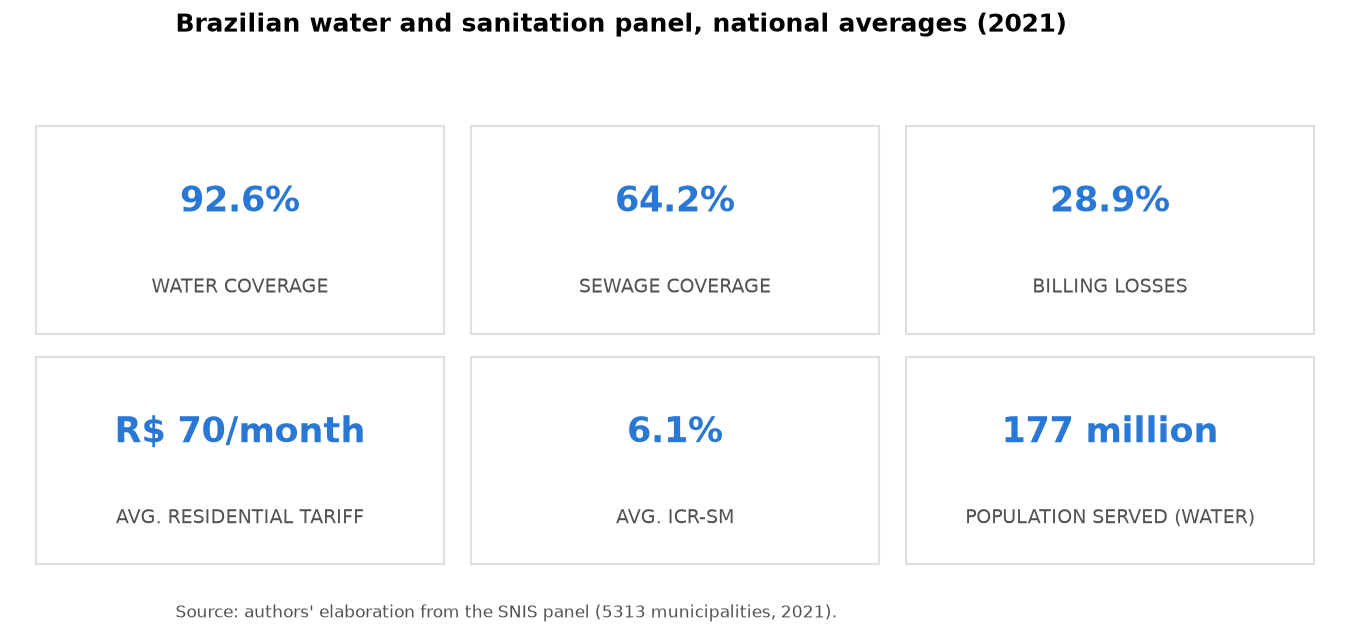
\includegraphics[width=0.85\textwidth]{../figuras/14_painel_numeros_nacionais.png}
\caption{Brazilian water and sanitation panel, national averages for the most recent year with complete data.}\label{fig_panel_stats}
\end{figure}

\paragraph{Affordability measure.}

For each municipality $i$ and year $t$, the average monthly residential bill is defined as

\begin{equation}
\text{Tariff}_{it} = \frac{\text{Revenue}^{water}_{it} + \text{Revenue}^{sewer}_{it}}{12 \times \text{Connections}_{it}}
\label{eq_tariff}
\end{equation}

where $\text{Revenue}^{water}_{it}$ and $\text{Revenue}^{sewer}_{it}$ are the direct operating revenue from water and sewer services and $\text{Connections}_{it}$ is the number of active residential connections. The affordability indicator, denoted ICR (income commitment ratio), is then

\begin{equation}
\text{ICR}_{it} = 100 \times \frac{\text{Tariff}_{it}}{W_{t}}
\label{eq_icr}
\end{equation}

where $W_{t}$ is a reference income floor, here the day weighted average national minimum wage in year $t$. The ICR-SM should be read as a municipal level proxy for the tariff burden carried by already connected customers, not as a direct household level measure of affordability or of customer equity. It represents the burden of the average bill relative to a national income floor rather than relative to the actual income of each household, it says nothing about households too poor or too remote to be connected in the first place, and it takes the same national reference wage for every municipality in a given year, so cross sectional differences in the indicator reflect differences in the average bill rather than in local income distribution. This adaptation is necessary because annual municipal household income data are not available for the full study period, and the resulting measure is best understood as an administrative tariff burden indicator that is informative about customer equity only to the extent that it varies with attributes, such as municipal size or region, plausibly correlated with the composition of the connected customer base. Equation~\eqref{eq_icr} can also use a regional or state level average wage $W_{st}$, which is examined as a robustness alternative. Observations with $\text{ICR}_{it}$ outside the $[0,100]$ range are treated as missing. They represent approximately 0.2 percent of the original panel and are more plausibly associated with underreporting of connections than with genuine unaffordability.

\paragraph{Planning and structural variables.}

Investment per capita is

\begin{equation}
\text{Inv}_{it} = \frac{\text{TotalInvestment}_{it}}{\text{PopulationServed}_{it}}
\label{eq_inv}
\end{equation}

Investment instability is measured by the coefficient of variation of $\text{Inv}_{it}$ over a trailing window of $w$ years,

\begin{equation}
\text{CV}^{w}_{it} = \frac{\sigma\left(\text{Inv}_{i,t-w},\ldots,\text{Inv}_{i,t-1}\right)}{\bar{\text{Inv}}\left(\text{Inv}_{i,t-w},\ldots,\text{Inv}_{i,t-1}\right)}
\label{eq_cv}
\end{equation}

with $w=5$ years as the main specification and $w \in \{3,10\}$ as robustness alternatives. The financing structure is captured by the share of investment funded through onerous, that is debt based, sources,

\begin{equation}
\text{Fin}_{it} = \frac{\text{OnerousFinancing}_{it}}{\text{TotalInvestment}_{it}}
\label{eq_fin}
\end{equation}

Billing losses enter as the reported loss index directly from the source panel. Municipal size and economic capacity are included as $\ln(\text{Population}_{it})$ and $\ln(\text{GDPperCapita}_{it})$. Population and services value added growth rates are computed as year over year percentage changes from the same underlying series.

\paragraph{Lag structure.}

All planning variables enter the affordability model in lagged form, using information available up to $t-1$, so that $\text{Inv}_{i,t-1}$, $\text{CV}^{w}_{i,t-1}$, $\text{Fin}_{i,t-1}$ and the lagged loss index predict $\text{ICR}_{it}$ rather than being observed in the same year as the outcome. This choice reflects the fact that tariffs and investment are typically set within the same annual budget cycle, so a contemporaneous specification would confound the direction of association between planning and price. A contemporaneous specification is estimated as a robustness check.

\subsection{Estimation and forecasting}\label{subsec_panel_spec}

The main model is a two way fixed effects panel regression,

\begin{equation}
Y_{it} = \mathbf{X}_{i,t-1}' \boldsymbol{\beta} + \mu_i + \lambda_t + \varepsilon_{it}
\label{eq_panel}
\end{equation}

where $Y_{it}$ is either $\text{ICR}_{it}$ or a coverage index, $\mathbf{X}_{i,t-1}$ collects the lagged planning and control variables defined above, $\mu_i$ is a municipality fixed effect absorbing all time invariant local characteristics, $\lambda_t$ is a year fixed effect absorbing shocks common to all municipalities in a given year, such as national inflation or a change in federal regulation, and $\varepsilon_{it}$ is an idiosyncratic error clustered at the municipality level. Model~\eqref{eq_panel} is estimated by the within estimator, and we report the within $R^2$, computed from the fit of the time demeaned model, alongside the between $R^2$, computed from an auxiliary regression of municipality level means on the means of the regressors, to decompose how much of the variance in $Y_{it}$ is explained by variation across municipalities as opposed to variation within the same municipality over time.

To test whether the coverage affordability relationship differs by region, the model is extended with an interaction term,

\begin{equation}
\text{ICR}_{it} = \beta_0 \, \text{Cov}_{it} + \sum_{r=1}^{R-1} \beta_r \left(\text{Cov}_{it} \times D_{ir}\right) + \mathbf{Z}_{it}' \boldsymbol{\gamma} + \mu_i + \lambda_t + \varepsilon_{it}
\label{eq_interaction}
\end{equation}

where $D_{ir}$ is a time invariant indicator for region $r$, one region held as the reference category, and $\mathbf{Z}_{it}$ collects controls. Because $D_{ir}$ alone is absorbed by $\mu_i$, only its interaction with the time varying coverage term is identified, which is the quantity of interest here.

\paragraph{Coverage projection to the legal target.}

For each municipality with at least three years of observed coverage, we fit an ordinary least squares trend

\begin{equation}
\text{Cov}_{it} = a_i + b_i \, t + u_{it}
\label{eq_trend}
\end{equation}

over the observed years and extrapolate to the target year $t^{*}$,

\begin{equation}
\widehat{\text{Cov}}_{i,t^{*}} = \hat{a}_i + \hat{b}_i \, t^{*}
\label{eq_extrapolation}
\end{equation}

Each municipality is then classified against a legal target $\tau$ with tolerance margin $m$,

\begin{equation}
\text{Status}_i =
\begin{cases}
\text{on track} & \text{if } \widehat{\text{Cov}}_{i,t^{*}} \geq \tau \\
\text{at risk} & \text{if } \tau - m \leq \widehat{\text{Cov}}_{i,t^{*}} < \tau \\
\text{will not meet} & \text{if } \widehat{\text{Cov}}_{i,t^{*}} < \tau - m
\end{cases}
\label{eq_classification}
\end{equation}

with $\tau = 99$ and $\tau = 90$ percent for water and sanitation respectively, $t^{*} = 2033$ and $m = 10$ percentage points, matching the legal thresholds stated in the introduction. This procedure requires only a coverage series of at least three years per unit and a numeric legal or policy target, and is directly transferable to any country with a stated universal access deadline.

\paragraph{Machine learning forecast and validation.}

The forecasting exercise calls for a different kind of model than the panel regressions above, one that predicts a future value rather than estimates an average partial effect, and the choice of model follows from that difference in task. Gradient boosted trees were selected over a linear forecasting model because the regressor set mixes a categorical variable, region, with continuous variables on very different scales and with plausible nonlinearities and interactions, for instance a given rate of population growth may matter differently for coverage depending on how large or how climatically exposed a municipality already is, relationships a tree based ensemble can represent without the functional form being specified in advance. The same choice was preferred over a neural network because the panel is tabular, moderate in size once restricted to complete cases, and gradient boosted trees are the established benchmark for tabular prediction tasks of this kind, typically matching or outperforming deep learning approaches on data of this structure while remaining far less demanding to tune and, through permutation importance, easier to inspect after fitting. The model is therefore best understood as the most flexible member of the model family still practical for this panel, so that if planning, economic or climate covariates carried predictive signal the linear panel specification could not capture, this design gives them the best available chance to show it.

\textit{Data treatment for the forecasting model.}

Before any series enters the forecasting model, the affordability and planning variables are built from the raw administrative panel, bounded or cleaned where implausible, and shifted to their $t-1$ lag. Three treatment choices are specific to the forecasting exercise. No feature scaling or normalization is applied because gradient boosted trees split on ranked feature values. Missing values are handled natively rather than imputed. The train and test partitions are split strictly by calendar year, never at random, so that no future observation is available during training. Figure~\ref{fig_ml_series} plots the national average trajectory of every series entering $\mathbf{X}_{i,t-1}$ and marks the boundary between the training years and the holdout years used for validation.

\begin{figure}[h]
\centering
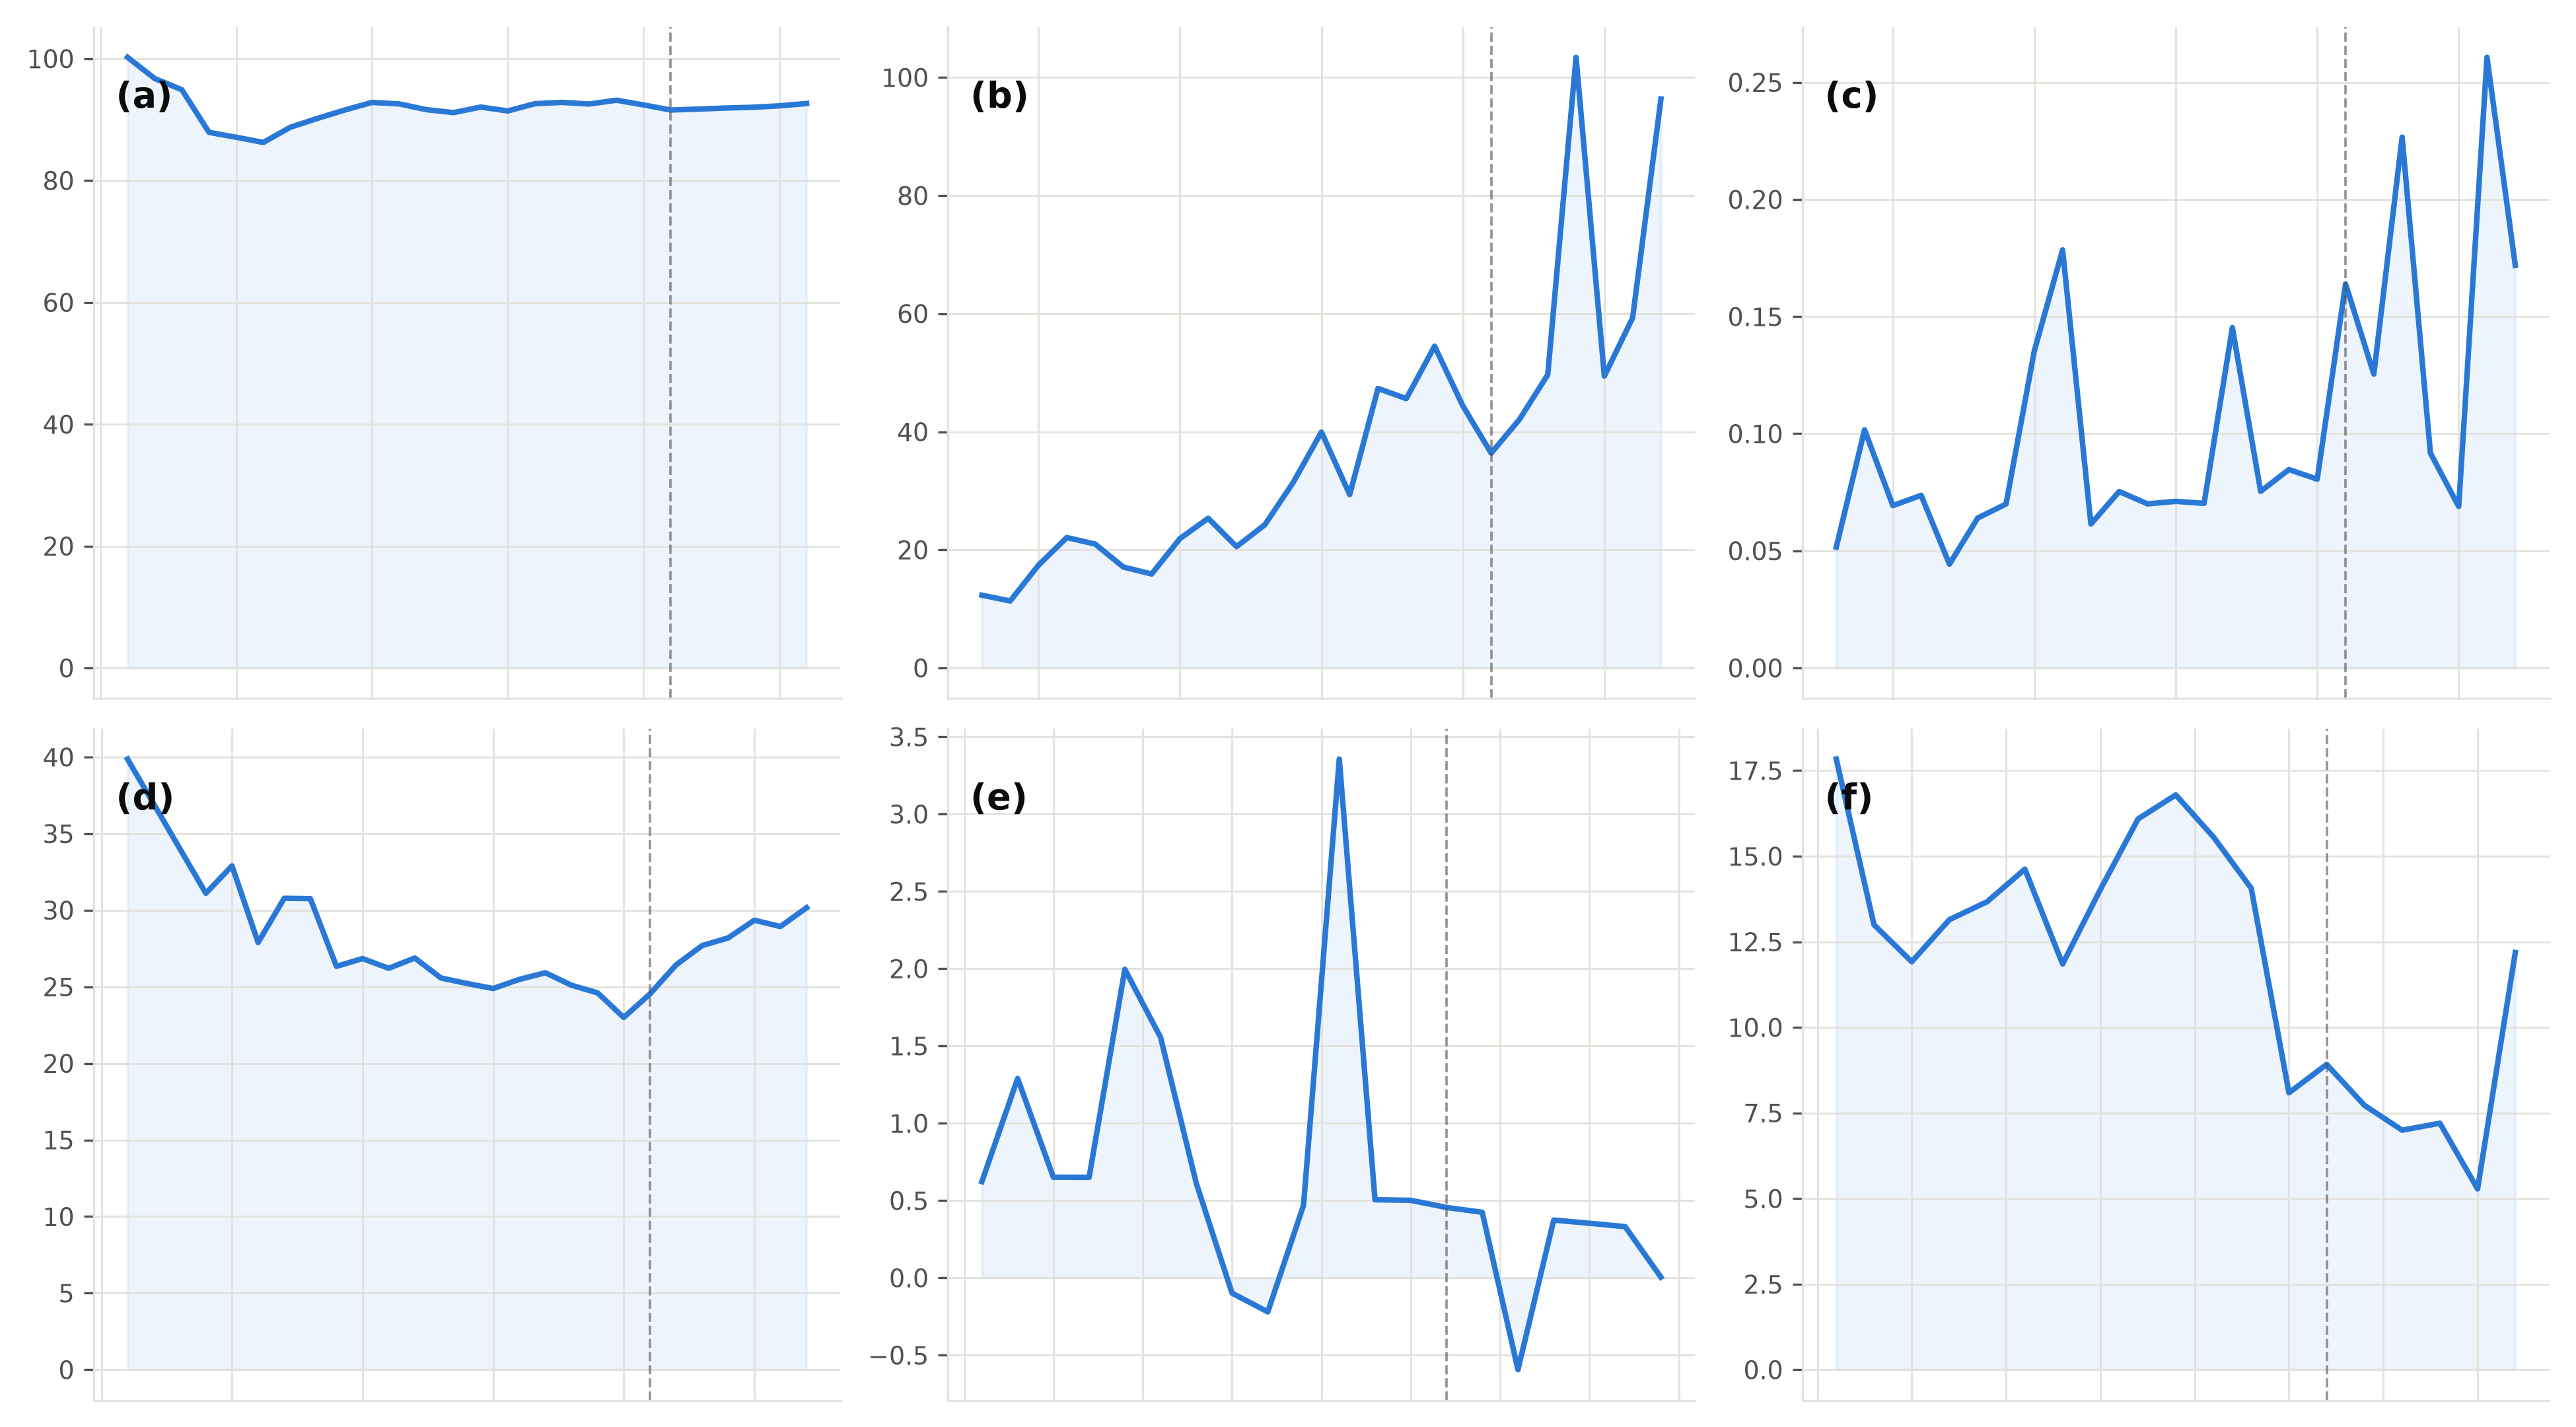
\includegraphics[width=\textwidth]{../figuras/15_series_temporais_ml.png}
\caption{National average trajectories of the variables used as regressors in the forecasting model, all covering the same period, 1995 to 2022, with the dashed vertical line marking the 2016/2017 boundary between the training years and the holdout years used for validation. Panel (a) is water coverage, panel (b) is investment per capita, panel (c) is the onerous financing share, panel (d) is the billing loss index, panel (e) is the population growth rate and panel (f) is the services value added growth rate.}\label{fig_ml_series}
\end{figure}

As an alternative to the linear trend of Equation~\eqref{eq_trend}, we train a one step ahead forecasting model

\begin{equation}
\widehat{\text{Cov}}_{it} = f\left(\text{Cov}_{i,t-1}, \mathbf{X}_{i,t-1}\right)
\label{eq_ml}
\end{equation}

where $f$ is a histogram based gradient boosting regressor fit by minimizing squared error loss, trained on years up to a cutoff and evaluated on a holdout period never seen during training. Concretely, $f$ is an ensemble of $300$ boosting iterations of depth up to $6$, with a learning rate of $0.05$, in which the region indicator enters as a native categorical split and missing covariate values are handled natively. The regressors are lagged investment per capita, lagged investment instability, lagged financing share, the lagged loss index, log population, log per capita GDP, population and services growth rates, region and the precipitation anomaly. The model is trained on all municipality year observations with $t \leq 2016$ and evaluated on the untouched holdout period $2017 \leq t \leq 2022$, so that no information from the evaluation years enters training either directly or through hyperparameter tuning. Forecast accuracy is reported using the mean absolute error and the root mean squared error,

\begin{equation}
\text{MAE} = \frac{1}{N}\sum_{i,t}\left|Y_{it}-\widehat{Y}_{it}\right|, \qquad
\text{RMSE} = \sqrt{\frac{1}{N}\sum_{i,t}\left(Y_{it}-\widehat{Y}_{it}\right)^{2}}
\label{eq_error}
\end{equation}

computed on the holdout period for three competing predictors, namely the trained model $f$, a naive persistence rule $\widehat{\text{Cov}}_{it}=\text{Cov}_{i,t-1}$, and the linear trend of Equation~\eqref{eq_trend} fit only on data available before $t$. To project beyond the last observed year, $f$ is applied recursively, feeding each year's forecast back in as the lagged coverage term for the following year, with investment and loss regressors held at their last observed value and growth rate regressors set to each municipality's long run compound annual growth rate computed over its full observed history. This recursive design generalizes to any panel with a lagged outcome and a set of slower moving covariates, provided a reasonable long run assumption for covariates beyond the observed sample can be specified. When the same recursive design is applied to affordability in Section~\ref{subsec_resultados5}, the population growth regressor is set instead to the state level population growth rate implied by the official IBGE population projection for 2022 to 2033, IBGE SIDRA table 7358\footnote{\url{https://sidra.ibge.gov.br/tabela/7358}}, since a municipality's own historical compound growth rate does not reflect Brazil's projected demographic deceleration over this specific horizon.

To assess which regressors the trained model relies on, an ablation is performed on the holdout period through permutation importance. Each covariate is independently shuffled across observations, five repetitions are performed per covariate, and the resulting change in holdout accuracy is recorded. A covariate whose permutation leaves accuracy unchanged, or improves it, provides no evidence of a genuine predictive contribution. The results are reported with the forecast evaluation.

\begin{table}[h]
\caption{Permutation importance of each covariate for the one step ahead coverage forecast, holdout period 2017--2022}\label{tab_ablation}
\begin{tabular}{@{}lc@{}}
\toprule
Covariate & Permutation importance \\
\midrule
Lagged coverage & 1,3030 \\
Region & 0,0035 \\
Population growth rate & 0,0019 \\
Year & 0,0000 \\
Lagged financing share & $-0{,}0002$ \\
Log per capita GDP & $-0{,}0003$ \\
Services growth rate & $-0{,}0004$ \\
Log population & $-0{,}0033$ \\
Lagged investment instability & $-0{,}0033$ \\
Precipitation anomaly & $-0{,}0075$ \\
Lagged investment per capita & $-0{,}0107$ \\
Lagged loss index & $-0{,}0219$ \\
\botrule
\end{tabular}
\footnotetext{Mean decrease in holdout $R^2$ across five random permutations per
covariate; negative values indicate no genuine contribution, within noise.}
\end{table}

\textit{A second forecasting model targeting affordability directly.}

The forecast described so far targets coverage, so it speaks to whether the same reported variables predict a different outcome, not to whether they forecast affordability itself. To close that gap, a second model of identical architecture is trained to forecast the affordability indicator one step ahead,

\begin{equation}
\widehat{\text{ICR}}_{it} = g\left(\text{ICR}_{i,t-1}, \mathbf{X}_{i,t-1}\right)
\label{eq_ml_icr}
\end{equation}

where $g$ uses the same hyperparameters, regressor set, categorical handling, training cutoff at 2016 and holdout period 2017 to 2022 as $f$ in Equation~\eqref{eq_ml}, with $\text{ICR}_{i,t-1}$ replacing $\text{Cov}_{i,t-1}$ as the autoregressive term. This gives the study a genuine machine learning forecast of affordability, evaluated with the same MAE and RMSE criteria of Equation~\eqref{eq_error} and the same permutation importance procedure, reported together with the panel results in Section~\ref{subsec_resultados2}. A random forest regressor, trained on the same one hot encoded regressors with missing values imputed at the training median, is estimated alongside $g$ wherever affordability is projected to 2033, so that the recursive forecast is checked against a second tree based ensemble that averages many independently bootstrapped trees rather than fitting one tree to the residuals of the last, a different source of variance reduction that behaves differently once errors are chained across many recursive steps. A recurrent neural network was considered for this forecasting task and set aside, each municipality contributes at most 28 annual observations, too short a sequence for a model class that typically needs long sequences per unit to learn temporal structure rather than memorize noise, so gradient boosting and random forest remain the two models compared throughout.

\paragraph{Robustness checks.}

The panel and forecasting results above are subjected to three further checks rather than taken at face value, with results reported together with the main findings in Section~\ref{sec2}. The panel model is reestimated with three and ten year windows in place of the five year window and with a contemporaneous version of the planning variables, to see whether the absence of a planning effect depends on the particular lag structure chosen, reported in Table~\ref{tab_robustez}. The affordability measure is separately reconstructed by replacing the national reference wage $W_t$ with a state year average wage $W_{st}$ drawn from an independent household survey, and the alternative outcome and the original outcome are then estimated on the same restricted sample, so that any shift in results can be traced to the income denominator rather than to the change in sample period. Finally, the correlation between each municipality's coverage trend slope $\hat{b}_i$ and its affordability trend slope is computed as a model free check on whether municipalities that gained coverage faster also lost affordability faster.

\paragraph{Software and reproducibility.}

All steps are implemented in a sequence of independent, numbered scripts, each reading clearly named input files and writing clearly named output files, so that the full pipeline can be rerun end to end or any single stage can be substituted. Panel construction and variable definitions use standard data manipulation routines, fixed effects estimation uses a panel regression package supporting two way fixed effects with cluster robust standard errors, and the machine learning forecast uses a histogram based gradient boosting implementation with native support for missing values. Applying the pipeline to a different country or a different administrative level requires the same functional data components assembled in the same panel format, with no change to the estimation code.

\section{Results}\label{sec2}

This section reports the empirical findings in the order the research questions were posed. It first describes how affordability varies across time, region and municipal size, establishing the descriptive pattern the rest of the section interprets. It then examines whether planning variables are associated with affordability once fixed effects are introduced, finds no robust association across specifications, and subjects that finding to a set of robustness checks and to a direct machine learning forecast of the affordability indicator itself. It then locates where a coverage affordability trade off does appear and how growth pressure divides between price and access effects, before closing with the joint trajectory of water and sanitation toward the legal deadline and an honest accounting of forecast uncertainty. Each part favors interpretation of what the reported statistics mean substantively, the full numerical detail is left to the accompanying tables.

\subsection{Affordability over time, space and municipal size}\label{subsec_resultados1}

The national median ICR-SM fell sharply in the first years of the panel and then settled into a narrow band from around 2010 onward, a plateau that already sits above the upper bound of the international affordability range of 3 to 5 percent. This trajectory is not obviously a planning achievement. It coincides with a period of sustained real appreciation of the minimum wage, so a meaningful share of the apparent improvement reflects the reference income rising faster than the tariff itself rather than more deliberate tariff design. The year fixed effects in the panel model absorb this common national trend, which is why the within municipality estimates presented next are the more informative test of whether planning matters.

The regional pattern runs against the intuitive expectation. The Northeast, the region with historically the weakest coverage, has the lowest median affordability burden in the country, while the South, with the strongest coverage, has the highest. Table~\ref{tab_icr_regiao} reports the full regional breakdown. The most plausible reading is that tariffs in the Northeast subsidize access more heavily, trading a lighter burden on connected households for a service that reaches fewer of them, while the South operates closer to full cost recovery. Municipal size follows a monotonic pattern instead, larger municipalities carry a systematically heavier burden, more than double that of the smallest municipalities, a relationship examined further once planning variables are controlled for below.

\begin{table}[h]
\caption{Median ICR-SM by region, 1995 to 2022 average}\label{tab_icr_regiao}
\begin{tabular}{@{}lccc@{}}
\toprule
Region & Median ICR-SM & Mean ICR-SM & N \\
\midrule
Northeast     & 4.8\% & 5.1\% & 30,430 \\
North         & 5.8\% & 6.4\% & 7,712 \\
Central West  & 6.5\% & 6.6\% & 8,467 \\
Southeast     & 7.1\% & 7.6\% & 28,805 \\
South         & 8.0\% & 8.2\% & 20,643 \\
\botrule
\end{tabular}
\end{table}

Figure~\ref{fig_mapa_icr} maps average ICR-SM by state and shows this regional pattern at finer resolution than the five official regions can convey, and reveals that the North is internally divided rather than uniformly light. Amazonas is the single lightest state in the country, and Maranhao, in the Northeast, sits almost as low, both well below their respective regional averages and consistent with small, isolated or heavily subsidized systems that charge little relative to the minimum wage. At the same time, two other North states, Rondonia and Amapa, are among the darkest in the country, closer to the southern states than to their regional neighbors, so the North average in Table~\ref{tab_icr_regiao} combines genuinely distinct tariff regimes rather than describing a single regional pattern. The Federal District is the single darkest unit on the map by a wide margin, roughly double the next highest state, a gap large enough that it is better read as a singular case, a wealthy, fully urbanized, single utility jurisdiction with a tariff structure geared to full cost recovery, than as representative of the Central West. Rio de Janeiro and Sao Paulo, in the Southeast, and Rio Grande do Sul, in the South, complete the group of states with the heaviest burden. This state level texture, with sharp within region contrasts sitting alongside the broader Northeast to South gradient, is the first piece of evidence, developed formally next, that affordability tracks conditions specific to where a household is rather than a small set of drivers that operate uniformly at the national or even the regional level.

\begin{figure}[h]
\centering
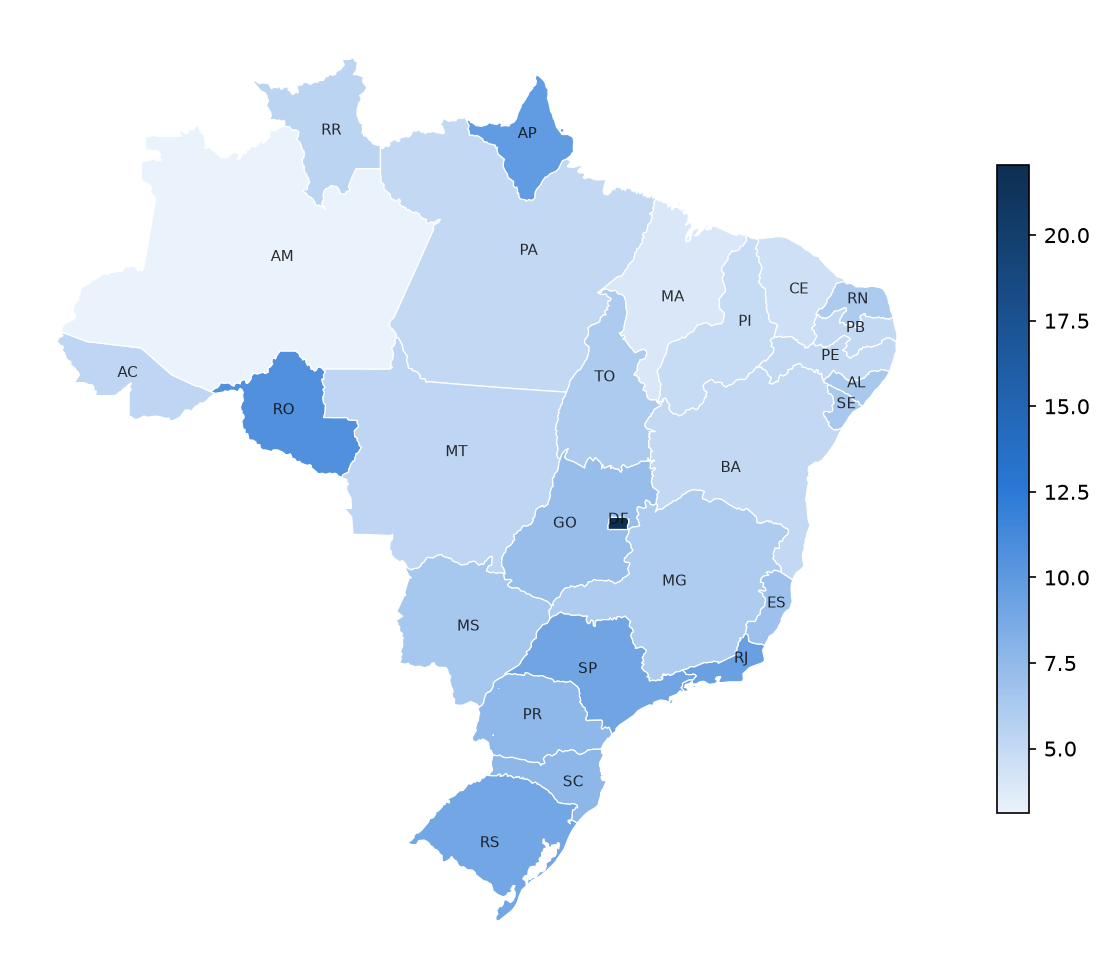
\includegraphics[width=0.75\textwidth]{../figuras/10_mapa_icr_sm_uf.png}
\caption{Average ICR-SM by state, 1995 to 2022. Darker shading indicates a heavier affordability burden.}\label{fig_mapa_icr}
\end{figure}

A second cut of the same data, by municipal population size rather than by place, gives the clearest municipal-size tariff-burden gradient in the panel. Table~\ref{tab_icr_porte} reports the median and mean ICR-SM for six size classes. The burden rises close to monotonically with size, from a median of 5.7 percent in municipalities under 5,000 residents to 12.2 percent in municipalities above 500,000, more than double, even though average reported water coverage is high, between 90 and 94 percent, in every size class and does not itself follow the same gradient. Because larger Brazilian municipalities concentrate a larger share of the country's minimum wage workforce, this gradient means that the households most exposed to a heavy tariff burden relative to the wage floor used here are disproportionately urban rather than rural, which cuts against a reading of Brazilian water affordability as chiefly a small town or remote area problem. This pattern is documented here rather than explained, since the size gradient could reflect full cost recovery pricing in larger, more autonomous utilities, a more diluted subsidy per connection in denser systems, or compositional differences in what counts as a residential connection in large metropolitan operators, and distinguishing between these mechanisms is left for future work with provider level detail this panel does not contain.

\begin{table}[h]
\caption{Median and mean ICR-SM by municipal population size class, 1995 to 2022 average}\label{tab_icr_porte}
\begin{tabular}{@{}lcccc@{}}
\toprule
Population size class & Median ICR-SM & Mean ICR-SM & Mean water coverage & N \\
\midrule
Under 5,000            & 5.7\% & 6.0\%  & 94.4\% & 34,041 \\
5,000 to 20,000        & 5.7\% & 6.3\%  & 90.1\% & 34,442 \\
20,000 to 50,000       & 7.0\% & 7.5\%  & 90.0\% & 11,790 \\
50,000 to 100,000      & 8.2\% & 8.7\%  & 90.3\% & 4,801 \\
100,000 to 500,000     & 9.8\% & 10.7\% & 92.9\% & 5,066 \\
Above 500,000          & 12.2\% & 13.4\% & 93.3\% & 904 \\
\botrule
\end{tabular}
\end{table}

\subsection{Planning variables show no robust within municipality association}\label{subsec_resultados2}

In the two way fixed effects model, none of the lagged planning variables, investment per capita, investment instability, the onerous financing share or the billing loss index, reaches conventional statistical significance, all with p values above 0.19. Non significance in a single specification is not proof that planning has no bearing on affordability, particularly with a one year lag, an annual reporting cadence and administrative variables that may not capture every planning relevant decision a utility makes, and it is read here together with a second, descriptive piece of evidence rather than in isolation. The between $R^2$, from an auxiliary regression of municipality level means on the means of the regressors, reaches 0.85, while the within $R^2$, from the time demeaned model, is close to zero. Taken jointly, the two results indicate that year to year movements in the four planning variables available in this panel carry little of the variation in the tariff burden, which is instead associated with whatever is fixed within a municipality across the study period. This is a statement about where the variance sits given the variables the sector reports about itself and the specification tested here, not a claim that municipal characteristics have been identified, that reverse causality and measurement error have been fully ruled out, or that planning is causally irrelevant under every possible measurement or longer lag structure.

This pattern recurs across alternative specifications rather than depending on one particular choice. Table~\ref{tab_robustez} repeats the estimation across four designs, varying the lag window used to compute investment instability and, as a stress test, removing the lag altogether. The last column of the table reports only the four planning variables themselves, investment per capita, investment instability, onerous financing and billing losses, so that its significance count is not confused with that of the municipal size control discussed below. The between $R^2$ stays in a narrow band from 0.85 to 0.87 throughout, and no planning variable is significant in any of the three lagged specifications. Planning variables do turn significant only in the contemporaneous design, which is also the specification most exposed to reverse causality, since tariffs and investment are typically decided within the same budget cycle. The signs recovered there, more losses associated with better affordability, are difficult to reconcile with a causal reading running from planning to outcome, and are more plausibly a symptom of that simultaneity than a genuine effect, which is why the lagged specifications are treated as the more informative ones.

\begin{table}[h]
	\caption{Robustness of the main model across four specifications, dependent variable ICR-SM}
	\label{tab_robustez}

	\begin{tabular*}{\textwidth}{@{\extracolsep{\fill}}>{\raggedright\arraybackslash}p{0.19\textwidth}cccc>{\raggedright\arraybackslash}p{0.22\textwidth}@{}}
		\toprule
		Specification & $N$ & Municipalities & $R^2$ \textit{between} &
		$R^2$ \textit{within} & Significant planning variables \\
		\midrule
		Original (lagged, 5 year CV)
		& 41,720 & 4,707 & 0.849 & $-0.013$ & none \\

		(a) Contemporaneous (no lag)
		& 44,889 & 4,740 & 0.853 & $-0.015$
		& Investment CV, losses \\

		(b) Lagged, 3 year CV window
		& 40,673 & 4,680 & 0.872 & $-0.015$ & none \\

		(c) Lagged, 10 year CV window
		& 37,057 & 4,552 & 0.871 & $-0.012$ & none \\

		\botrule
	\end{tabular*}
\end{table}

Municipal size carries a consistent secondary effect across most specifications, significant at 5 percent in three of the four, with p equal to 0.066 in the original one, larger municipalities tend toward a worse ICR-SM even after controlling for planning and fixed effects, in line with the descriptive pattern already noted above. This control is reported separately here precisely because it is a municipal characteristic rather than a planning choice, and its significance does not offset or contradict the absence of a planning effect documented in the same table.

The null result documented above describes the full 1995 to 2022 panel, but it is not temporally uniform, and that non uniformity is reported directly rather than folded into a single summary statistic. Table~\ref{tab_periodo_2012_2022} repeats the same coefficients for three specifications, the full panel, the 2012 to 2022 sub-period using the original ICR-SM, and the same sub-period using an alternative income denominator built from state level average wages rather than the single national minimum wage, available only from 2012 onward. The onerous financing share turns significant in both 2012 to 2022 specifications, with a sign opposite to what the original hypothesis anticipated, more debt associated with a lighter burden rather than a heavier one, and investment instability turns significant only under the alternative denominator. Because the onerous financing share is already significant in the 2012 to 2022 column that still uses the original ICR-SM, the divergence is attributable mainly to the shorter, more recent time window rather than to the choice of income denominator. A plausible reading, not tested directly here, is that the 2010s included subsidized financing programs for sanitation, so an onerous classification in that decade may have captured subsidized credit that enabled efficiency gains rather than the costly debt burden the original hypothesis assumed. The null result predominates across the full panel, but it is not temporally uniform, and the emergence of these associations in the most recent decade is reported as an open question about that period, plausibly reflecting institutional or financing changes specific to it, rather than as a resolved exception to the full panel result.

\begin{table}[h]
\caption{Planning variable coefficients with clustered standard errors, dependent variable ICR-SM unless noted, full panel and 2012 to 2022}\label{tab_periodo_2012_2022}
\begin{tabular}{@{}lccc@{}}
\toprule
 & Full panel & 2012--2022 & 2012--2022 \\
 & 1995--2022 & (ICR-SM) & (state income denominator) \\
\midrule
Investment per capita (lag)     & $-0.00002$ & $-0.00002$ & $-0.00003$ \\
                                 & \scriptsize$(0.00004)$ & \scriptsize$(0.00006)$ & \scriptsize$(0.00002)$ \\
Investment instability (lag)    & $-0.015$   & $-0.024$   & $-0.027^{**}$ \\
                                 & \scriptsize$(0.026)$ & \scriptsize$(0.024)$ & \scriptsize$(0.009)$ \\
Onerous financing share (lag)   & $0.035$    & $-0.187^{***}$ & $-0.072^{***}$ \\
                                 & \scriptsize$(0.036)$ & \scriptsize$(0.039)$ & \scriptsize$(0.013)$ \\
Billing loss index (lag)        & $-0.001$   & $-0.0004$  & $0.0001$ \\
                                 & \scriptsize$(0.001)$ & \scriptsize$(0.001)$ & \scriptsize$(0.0003)$ \\
\midrule
$N$              & 41,720 & 29,150 & 25,846 \\
Municipalities   & 4,707  & 4,475  & 4,433 \\
\botrule
\end{tabular}
\footnotetext{Standard errors clustered at the municipality level in parentheses. $^{**}p<0.01$, $^{***}p<0.001$; coefficients without a star are not significant at the 5 percent level. The state income denominator column uses a state year average wage from the PNADC household survey in place of the national minimum wage.}
\end{table}

A gradient boosting model of Equation~\eqref{eq_ml_icr} and a random forest of identical regressor set were trained to forecast the affordability indicator itself one year ahead, using the same chronological holdout as the coverage forecast described in Section~\ref{subsec_panel_spec}, so that this exercise, unlike the coverage forecast, tests the panel finding directly rather than by analogy. Table~\ref{tab_validacao_ml_icr} reports the result. As with coverage, both trained models are outperformed by the naive rule of repeating each municipality's last observed value, though all three are far more accurate than a per municipality linear extrapolation. This is a second empirical route, prediction rather than estimation, reaching a result consistent with the panel finding above, the year to year movement in the four planning variables carries little enough information about affordability that two different flexible models, each given every advantage over a simple persistence rule, still cannot use it profitably.

\begin{table}[h]
\caption{One year ahead validation of the affordability forecast, 2017 to 2022, mean absolute error of ICR-SM}\label{tab_validacao_ml_icr}
\begin{tabular}{@{}lcc@{}}
\toprule
Method & MAE (p.p.) & RMSE (p.p.) \\
\midrule
Persistence (repeats the last value)  & 0.48 & 1.26 \\
Random forest (ML)                    & 0.54 & 1.29 \\
Gradient boosting (ML)                & 0.56 & 1.28 \\
Linear extrapolation per municipality & 1.97 & 2.89 \\
\botrule
\end{tabular}
\end{table}

Permutation importance on this model, reported in Table~\ref{tab_ablation_icr}, shows one qualitative difference from the coverage forecast. The lagged affordability indicator still dominates by a wide margin, but log per capita GDP, lagged investment per capita, the lagged loss index and the investment instability window all show a small positive contribution, in contrast to the uniformly negative or negligible importances found for coverage. The contribution is modest, each of these covariates degrades holdout accuracy by well under one percent of what removing the lagged indicator itself would cost, so it does not overturn the panel result that none of the four planning variables is individually significant, but it is consistent with a weak, genuine, non zero signal running from local economic conditions and investment level to future affordability that the linear fixed effects specification, with its stricter functional form and one year lag, is not positioned to detect. Figure~\ref{fig_pred_obs_icr} shows the individual predictions behind Table~\ref{tab_validacao_ml_icr}, and the same compression pattern documented for coverage recurs here, the gradient boosting model tracks the persistence baseline closely through the middle of the distribution and departs from the 45 degree line mainly at the highest observed values of ICR-SM, where it pulls predictions back toward the bulk of the distribution.

\begin{table}[h]
\caption{Permutation importance of each covariate for the one step ahead affordability forecast, holdout period 2017--2022}\label{tab_ablation_icr}
\begin{tabular}{@{}lc@{}}
\toprule
Covariate & Permutation importance \\
\midrule
Lagged ICR-SM & 1.371 \\
Log per capita GDP & 0.015 \\
Lagged investment per capita & 0.009 \\
Lagged loss index & 0.004 \\
Population growth rate & 0.003 \\
Log population & 0.002 \\
Region & 0.002 \\
Lagged investment instability & 0.001 \\
Year & 0.000 \\
Lagged financing share & $-0.001$ \\
Services growth rate & $-0.001$ \\
Precipitation anomaly & $-0.002$ \\
\botrule
\end{tabular}
\footnotetext{Mean decrease in holdout $R^2$ across five random permutations per
covariate; negative values indicate no genuine contribution, within noise.}
\end{table}

\begin{figure}[h]
\centering
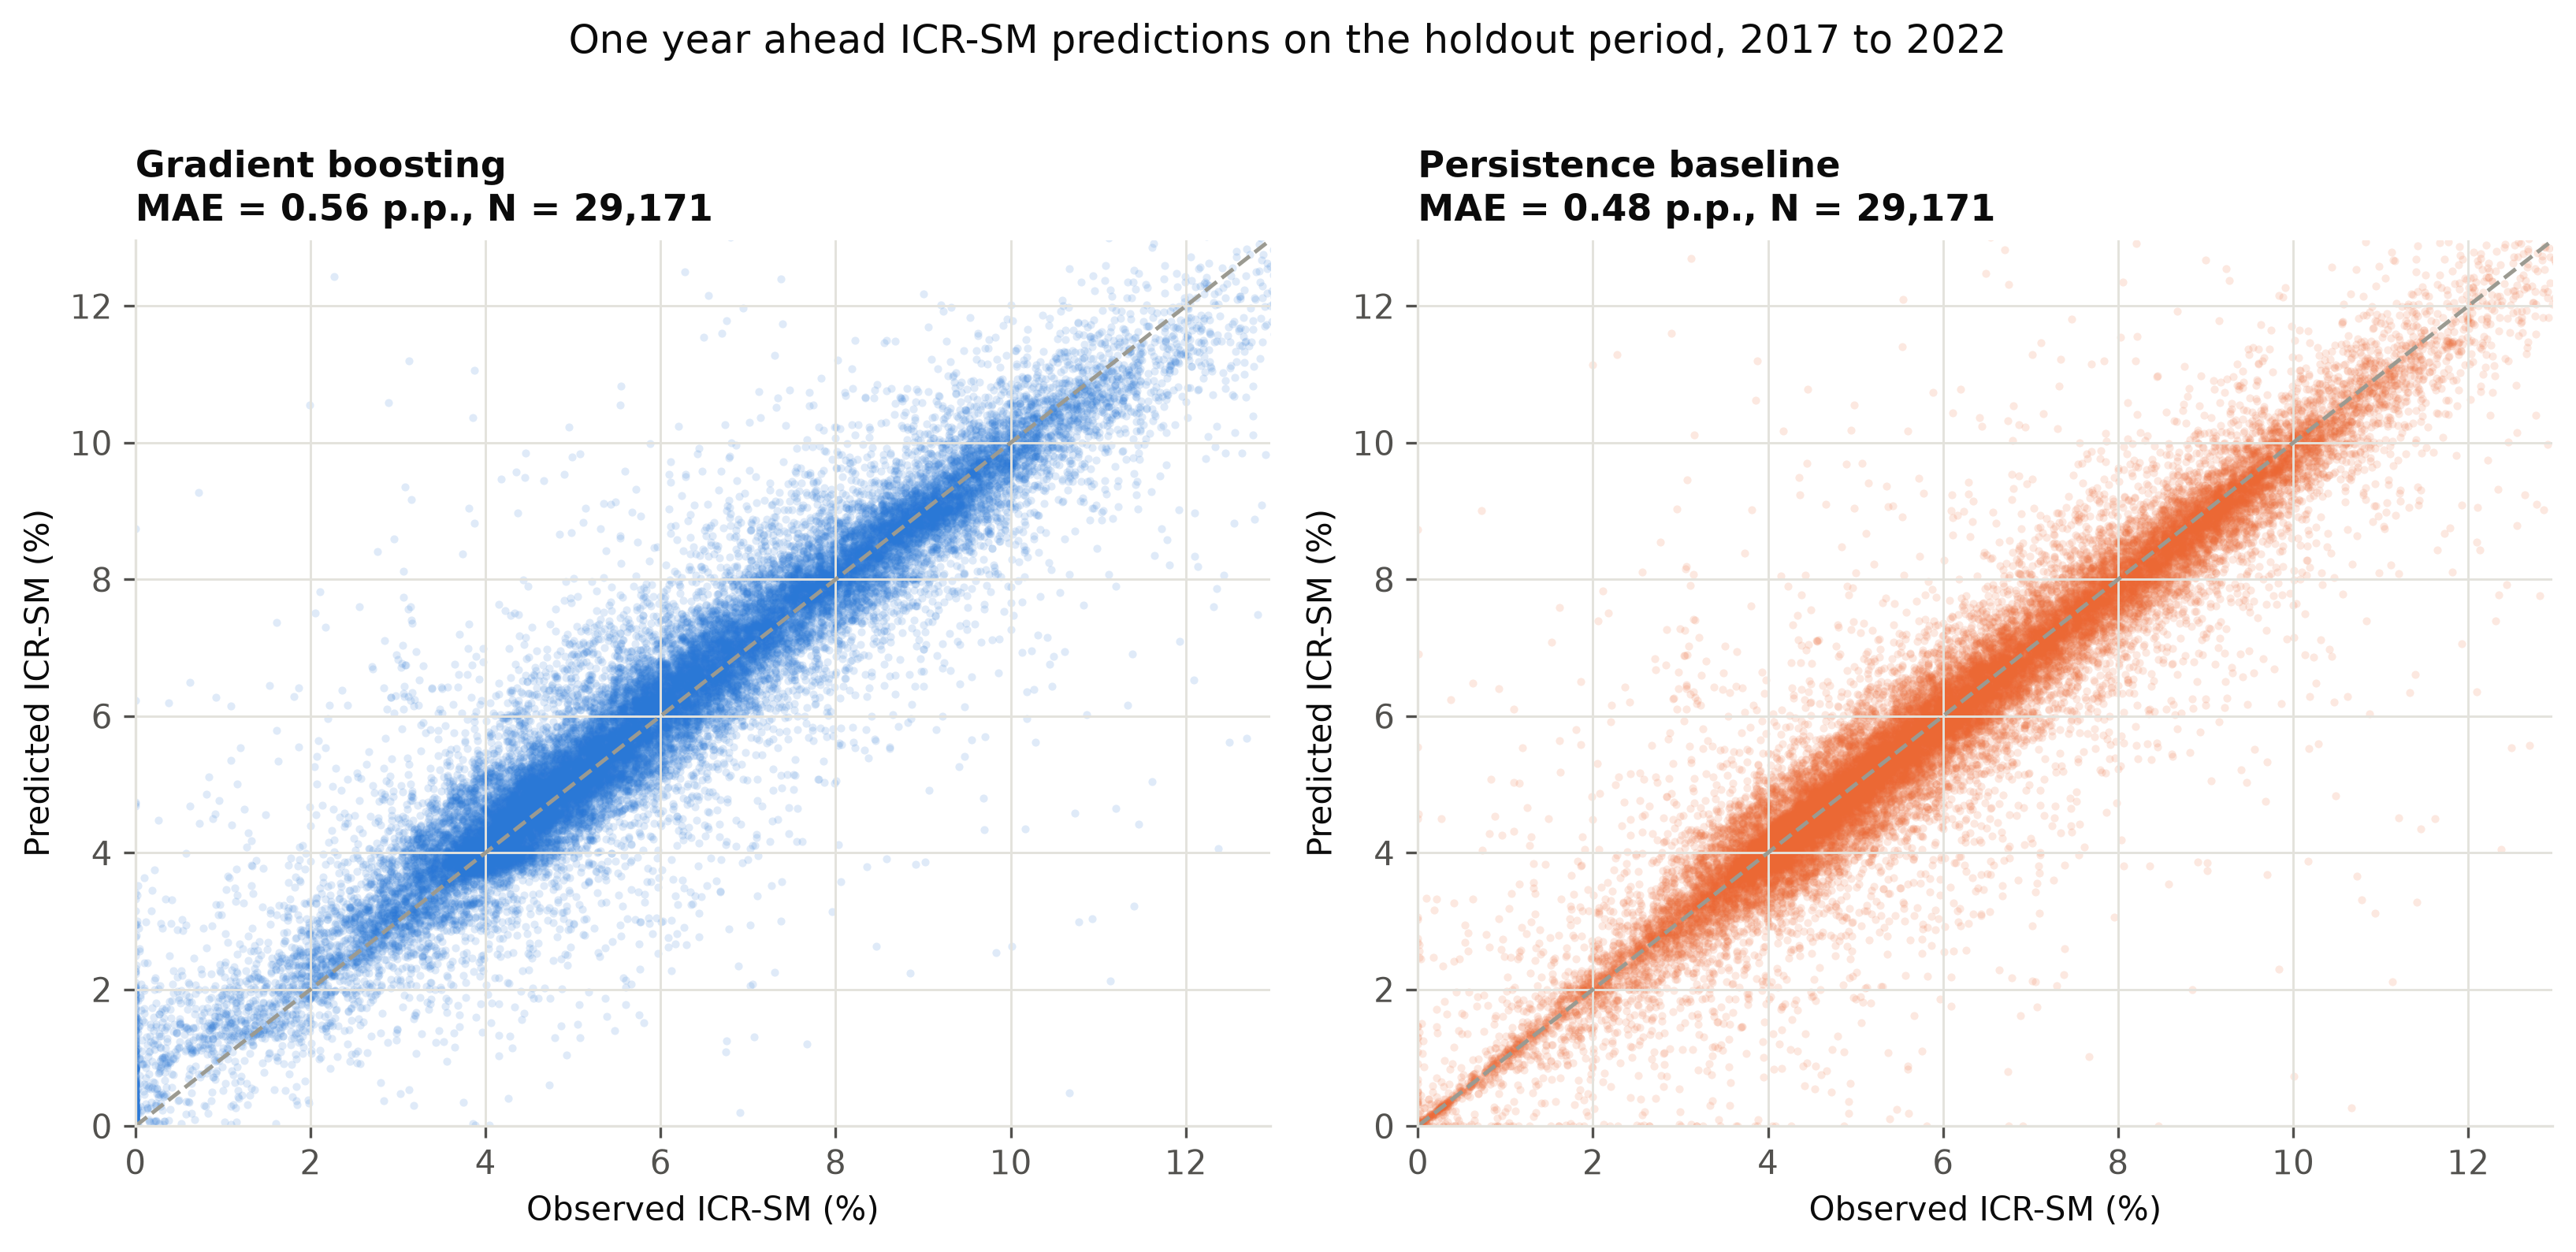
\includegraphics[width=\textwidth]{../figuras/18_previsto_vs_observado_icr.png}
\caption{Predicted against observed ICR-SM for every municipality year in the holdout period, 2017 to 2022, gradient boosting on the left and the persistence baseline on the right. The dashed line marks perfect prediction.}\label{fig_pred_obs_icr}
\end{figure}

\subsection{Where a coverage affordability trade off and growth pressure appear}\label{subsec_resultados3}

Two further tests locate where the system departs from the pattern of no detectable within municipality association documented above, one geographic and one dynamic. Interacting water coverage with region, using the Southeast as the reference category, shows that coverage is associated with lower ICR-SM in the Southeast itself. The interactions with the North and the Central West are positive and significant instead, meaning that in those two regions coverage gains arrive together with a worsening affordability burden. The interaction with the Northeast is not significant, so the region with historically the weakest coverage does not display the same trade off. This result qualifies rather than confirms the idea of a generic coverage affordability trade off, the tension is real, but it is concentrated in two specific regions and does not generalize to every region that has been expanding access.

The second departure concerns growth rather than region. Population growth reduces water coverage with a coefficient that is both economically and statistically meaningful, while its effect on affordability itself is not statistically distinguishable from zero. Growth in services value added, used here as a proxy for local economic dynamism, is associated with better affordability rather than worse, plausibly because a larger base of paying residential connections and greater ability to pay dilute fixed costs faster than it raises demand for network expansion. Read together, these two results support a division of labor in how growth pressure is absorbed by the system, it strains the access side, not the price side, which is consistent with the annual planning variables tested here showing no detectable association with affordability while coverage remains sensitive to how fast a municipality is growing.

\subsection{Water and sanitation trajectories toward 2033 and forecast uncertainty}\label{subsec_resultados5}

A municipality level linear extrapolation of historical coverage trends, based on the 5,431 of 5,549 municipalities with a usable water coverage series, classifies the majority as on track for the legal water coverage target of 99 percent by 2033, with a substantial minority at risk or projected not to meet it. The regional gap in this projection is wide, the share of municipalities projected to miss the water target in the South is a fraction of the corresponding share in the North, as reported in Table~\ref{tab_2033}.

Sanitation tells a different and more precarious story. A usable coverage series exists for only 2,971 of the 5,549 municipalities, roughly half the water figure, and the shortfall in reporting is itself informative, since municipalities that fail to report sanitation coverage tend to be the ones with weaker infrastructure to begin with, so the sanitation figures below are likely optimistic. Among municipalities that do report, the share projected to miss the sanitation target is roughly double the corresponding share for water. Strikingly, the South, the clear leader on water, has a share of municipalities projected to miss the sanitation target that approaches the Northeast's shortfall on water. Among municipalities on track for water, the majority are projected to miss the sanitation target, which means coverage of one service carries little information about coverage of the other.

\begin{table}[h]
\caption{Projected coverage status by 2033, by region, percent of municipalities}\label{tab_2033}
\begin{tabular*}{\textwidth}{@{\extracolsep\fill}lcccc}
\toprule
& \multicolumn{2}{@{}c@{}}{Water (99 percent target)} & \multicolumn{2}{@{}c@{}}{Sanitation (90 percent target)} \\
\cmidrule{2-3}\cmidrule{4-5}
Region & On track & Will not meet & On track & Will not meet \\
\midrule
South         & 83.5\% & 6.2\%  & 38.3\% & 53.5\% \\
Southeast     & 48.8\% & 27.6\% & 51.1\% & 38.9\% \\
Central West  & 45.1\% & 14.3\% & 38.8\% & 50.5\% \\
Northeast     & 50.6\% & 32.9\% & 31.3\% & 65.3\% \\
North         & 49.4\% & 37.0\% & 24.4\% & 73.1\% \\
\botrule
\end{tabular*}
\end{table}

Figure~\ref{fig_mapa_gap} maps this asymmetry by state, showing the difference between the projected sanitation shortfall and the projected water shortfall. Mato Grosso do Sul is the single most extreme case in the country, its sanitation shortfall roughly ten times its water shortfall, on a sample of 65 municipalities large enough to trust. Behind it, a cluster of states with reliable sanitation data, Sao Paulo, Rio de Janeiro and Rio Grande do Sul in the Southeast and South, and Bahia in the Northeast, all show sanitation lagging water by a wide margin, so the sanitation specific delay is not confined to any single region. The states where water instead appears to lag sanitation are concentrated in the North, but this reading needs an explicit caveat, several of them, including Acre, Amapa, Roraima and Amazonas, have fewer than ten municipalities with usable sanitation data, so their negative values are as much a symptom of sparse reporting as of a genuine reversal of the usual pattern. Maranhao is the one state in this group with a sample large enough, 26 municipalities, to read with more confidence, and it does show a real water lag relative to sanitation. Read together with Table~\ref{tab_2033}, the map reinforces that sanitation planning cannot be inferred from water planning even within the same state, let alone the same region.

\begin{figure}[h]
\centering
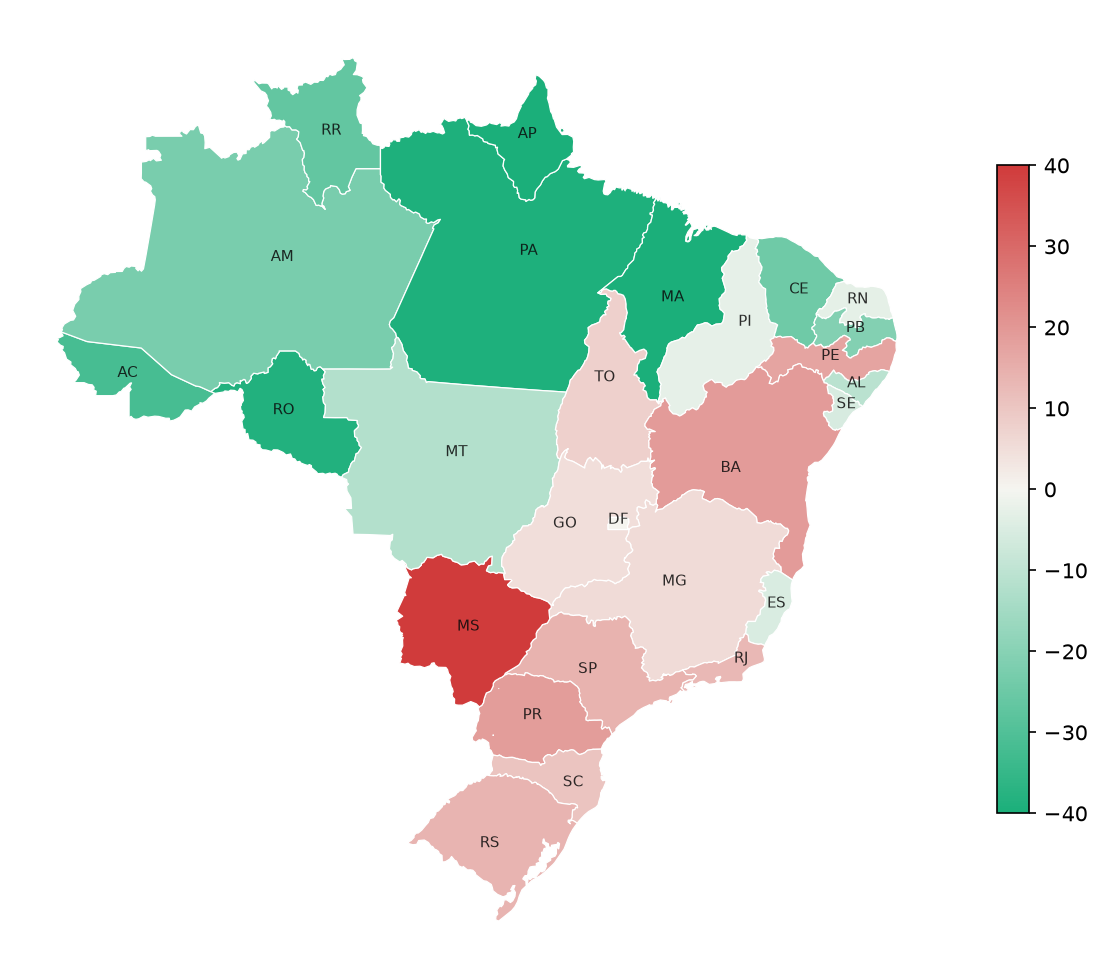
\includegraphics[width=0.85\textwidth]{../figuras/13_mapa_gap_agua_esgoto_uf.png}
\caption{Difference, in percentage points, between the share of municipalities projected to miss the sanitation target and the share projected to miss the water target, by state. Positive values, shown in red, indicate sanitation lagging water, negative values, shown in green, indicate the reverse.}\label{fig_mapa_gap}
\end{figure}

A further, model free test asks whether municipalities that gained coverage faster over the period also lost affordability faster, the direct test of a dynamic trade off. The correlation between each municipality's coverage trend slope and its affordability trend slope is close to zero and carries no statistical signal, so there is no evidence of a systematic long run trade off between expanding coverage and containing tariffs.

Finally, the reliability of the 2033 projection itself was evaluated by comparing the linear extrapolation against a gradient boosting model trained to forecast coverage one year ahead on 25,978 municipality year observations from 2017 to 2022, using only years up to and including 2016 for training, and then projected forward recursively. In that validation, reported in Table~\ref{tab_validacao_ml}, the machine learning model was outperformed by the simplest possible baseline, repeating the last observed value, which reinforces that infrastructure coverage carries strong structural inertia and is only weakly sensitive to planning variables even at a one year horizon. When both methods are projected out to 2033, they agree on only about a third of municipalities, with a sizable average gap between their level projections. The linear extrapolation is reported as the central scenario because it is more interpretable, but this disagreement should be read as genuine uncertainty about an eleven year trajectory rather than as a defect of one method relative to the other.

\begin{table}[h]
\caption{One year ahead validation, 2017 to 2022, mean absolute error of water coverage}\label{tab_validacao_ml}
\begin{tabular}{@{}lcc@{}}
\toprule
Method & MAE (p.p.) & RMSE (p.p.) \\
\midrule
Persistence (repeats the last value) & 2.16 & 8.83 \\
Gradient boosting (ML)               & 3.26 & 8.93 \\
Linear extrapolation per municipality & 6.47 & 14.45 \\
\botrule
\end{tabular}
\end{table}

Figure~\ref{fig_pred_obs} shows the individual predictions behind these summary statistics rather than the aggregate error alone. The persistence baseline, right panel, hugs the 45 degree line almost everywhere, which is exactly what is expected when a series changes little from one year to the next, last year's value is already close to the correct answer. The gradient boosting model, left panel, is visibly less faithful to that line, it systematically pulls predictions for municipalities with very low or very high observed coverage back toward the middle of the distribution, a compression pattern typical of tree based models when a single lagged feature dominates the fit, as it does here, and one that a simple average error number does not reveal on its own. The scatter therefore shows directly why the more flexible model does not help, it is not making sharper predictions than persistence, it is making systematically blunter ones at the extremes of the coverage distribution.

\begin{figure}[h]
\centering
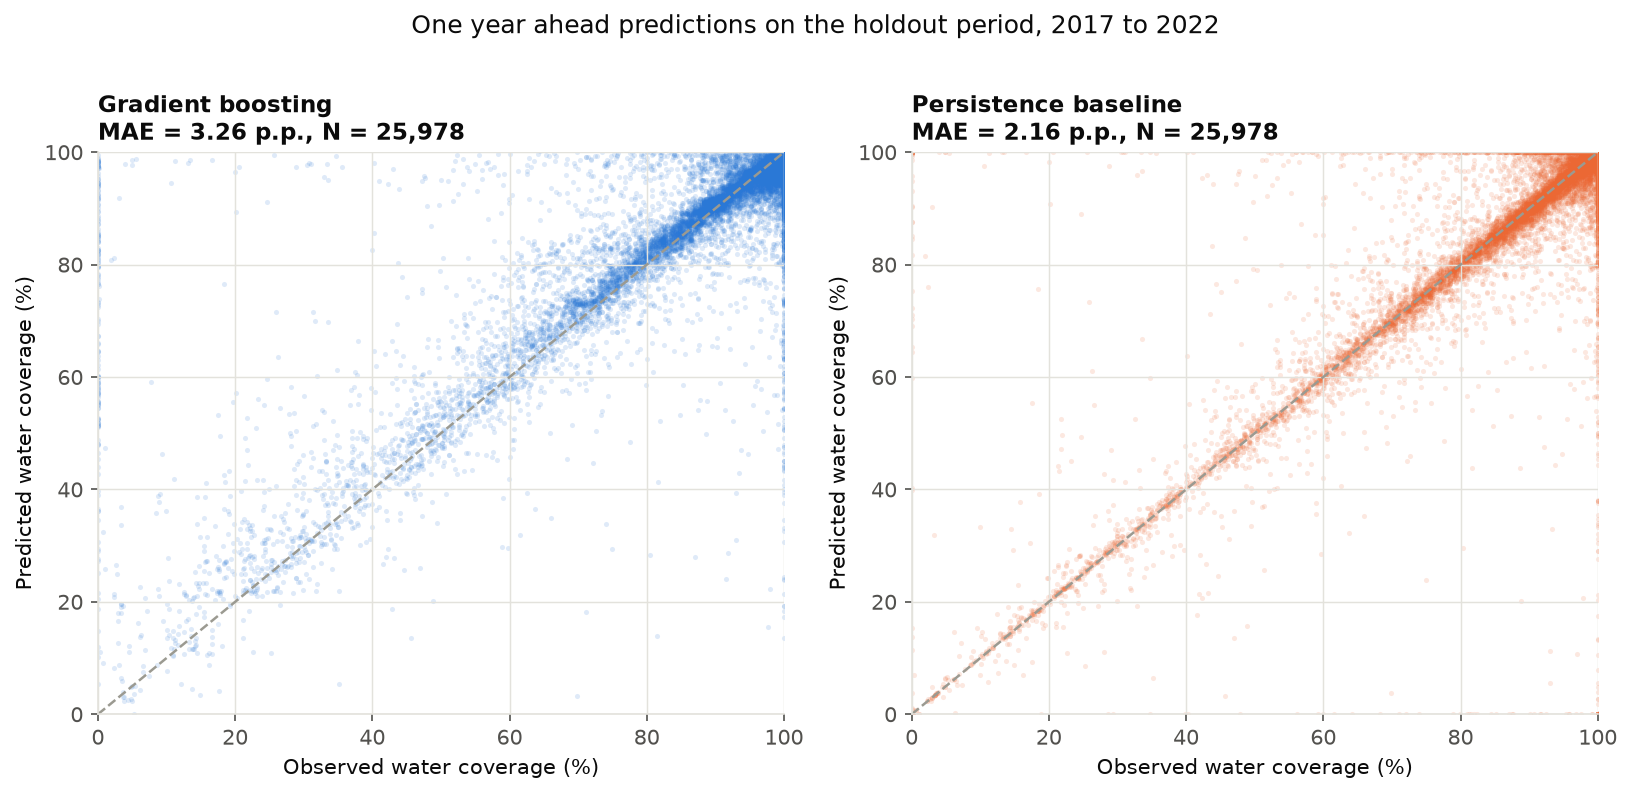
\includegraphics[width=\textwidth]{../figuras/16_previsto_vs_observado.png}
\caption{Predicted against observed water coverage for every municipality year in the holdout period, 2017 to 2022, gradient boosting on the left and the persistence baseline on the right. The dashed line marks perfect prediction.}\label{fig_pred_obs}
\end{figure}

\paragraph{What the affordability trajectory to 2033 could look like.}

Every projection reported so far targets coverage, which has a legal deadline but leaves open the question this special issue is ultimately about, what happens to the tariff burden itself over the same horizon. Three methods are applied here directly to the ICR-SM, a per municipality linear extrapolation and two recursive machine learning models, gradient boosting and random forest, each starting from every municipality's last observed value, with the population growth regressor set to the official IBGE population projection for 2022 to 2033 rather than each municipality's own historical growth rate, described in Section~\ref{subsec_panel_spec}. The three are reported as separate sensitivity scenarios rather than combined into a single estimate or range, precisely because they disagree in direction, not only in magnitude, and averaging across a decline and two increases would manufacture a false consensus. None of the three should be read as a validated eleven year forecast, the one year ahead validation in Table~\ref{tab_validacao_ml_icr} says nothing about accuracy once a model's own predictions are fed back into itself for eleven consecutive years, a known fragility of recursive forecasting, and the linear scenario simply continues each municipality's own historical slope with no validation step at all.

\begin{table}[h]
\caption{National ICR-SM in 2033 under three conditional scenarios}\label{tab_icr_2033_regiao}
\begin{tabular}{@{}lll@{}}
\toprule
Method & National ICR-SM in 2033 & Interpretation \\
\midrule
Linear trend        & 4.5\% & Continuation of the historical trajectory \\
Recursive random forest    & 6.0\% & Moderate reversal scenario \\
Recursive gradient boosting & 7.0\% & Sharper reversal scenario \\
\botrule
\end{tabular}
\end{table}

Figure~\ref{fig_icr_2033} plots the three trajectories against the observed series back to 1995. The linear scenario continues the gradual decline visible since the mid 2000s, inheriting two decades of real minimum wage appreciation outpacing tariff growth, documented in Section~\ref{subsec_resultados1}, an assumption that holds only if that policy pattern persists. Both recursive models instead reverse the recent trajectory, by different amounts, because they compound an estimated one year relationship across eleven consecutive iterations rather than continue a historical slope, so any bias in the last observed year's relationship between the lagged indicator and its covariates is repeated rather than averaged out. That the two recursive models disagree with each other, not only with the linear scenario, is itself informative, gradient boosting fits each new tree to the residuals of the last and can extrapolate a trend further, while random forest averages many independently bootstrapped trees, a form of averaging that tends to pull recursive forecasts toward a stable point rather than let them drift, visible in Figure~\ref{fig_icr_2033} as the random forest trajectory flattening after a few years while the gradient boosting trajectory keeps climbing. Two municipality level results feeding into the linear scenario are unstable enough to note briefly, the Federal District, a single municipality UF, and several municipalities in Mato Grosso do Sul receive linear extrapolations far outside any nationally observed value, a reminder that the linear scenario is the least numerically stable of the three at the tails of the distribution.

\begin{figure}[h]
\centering
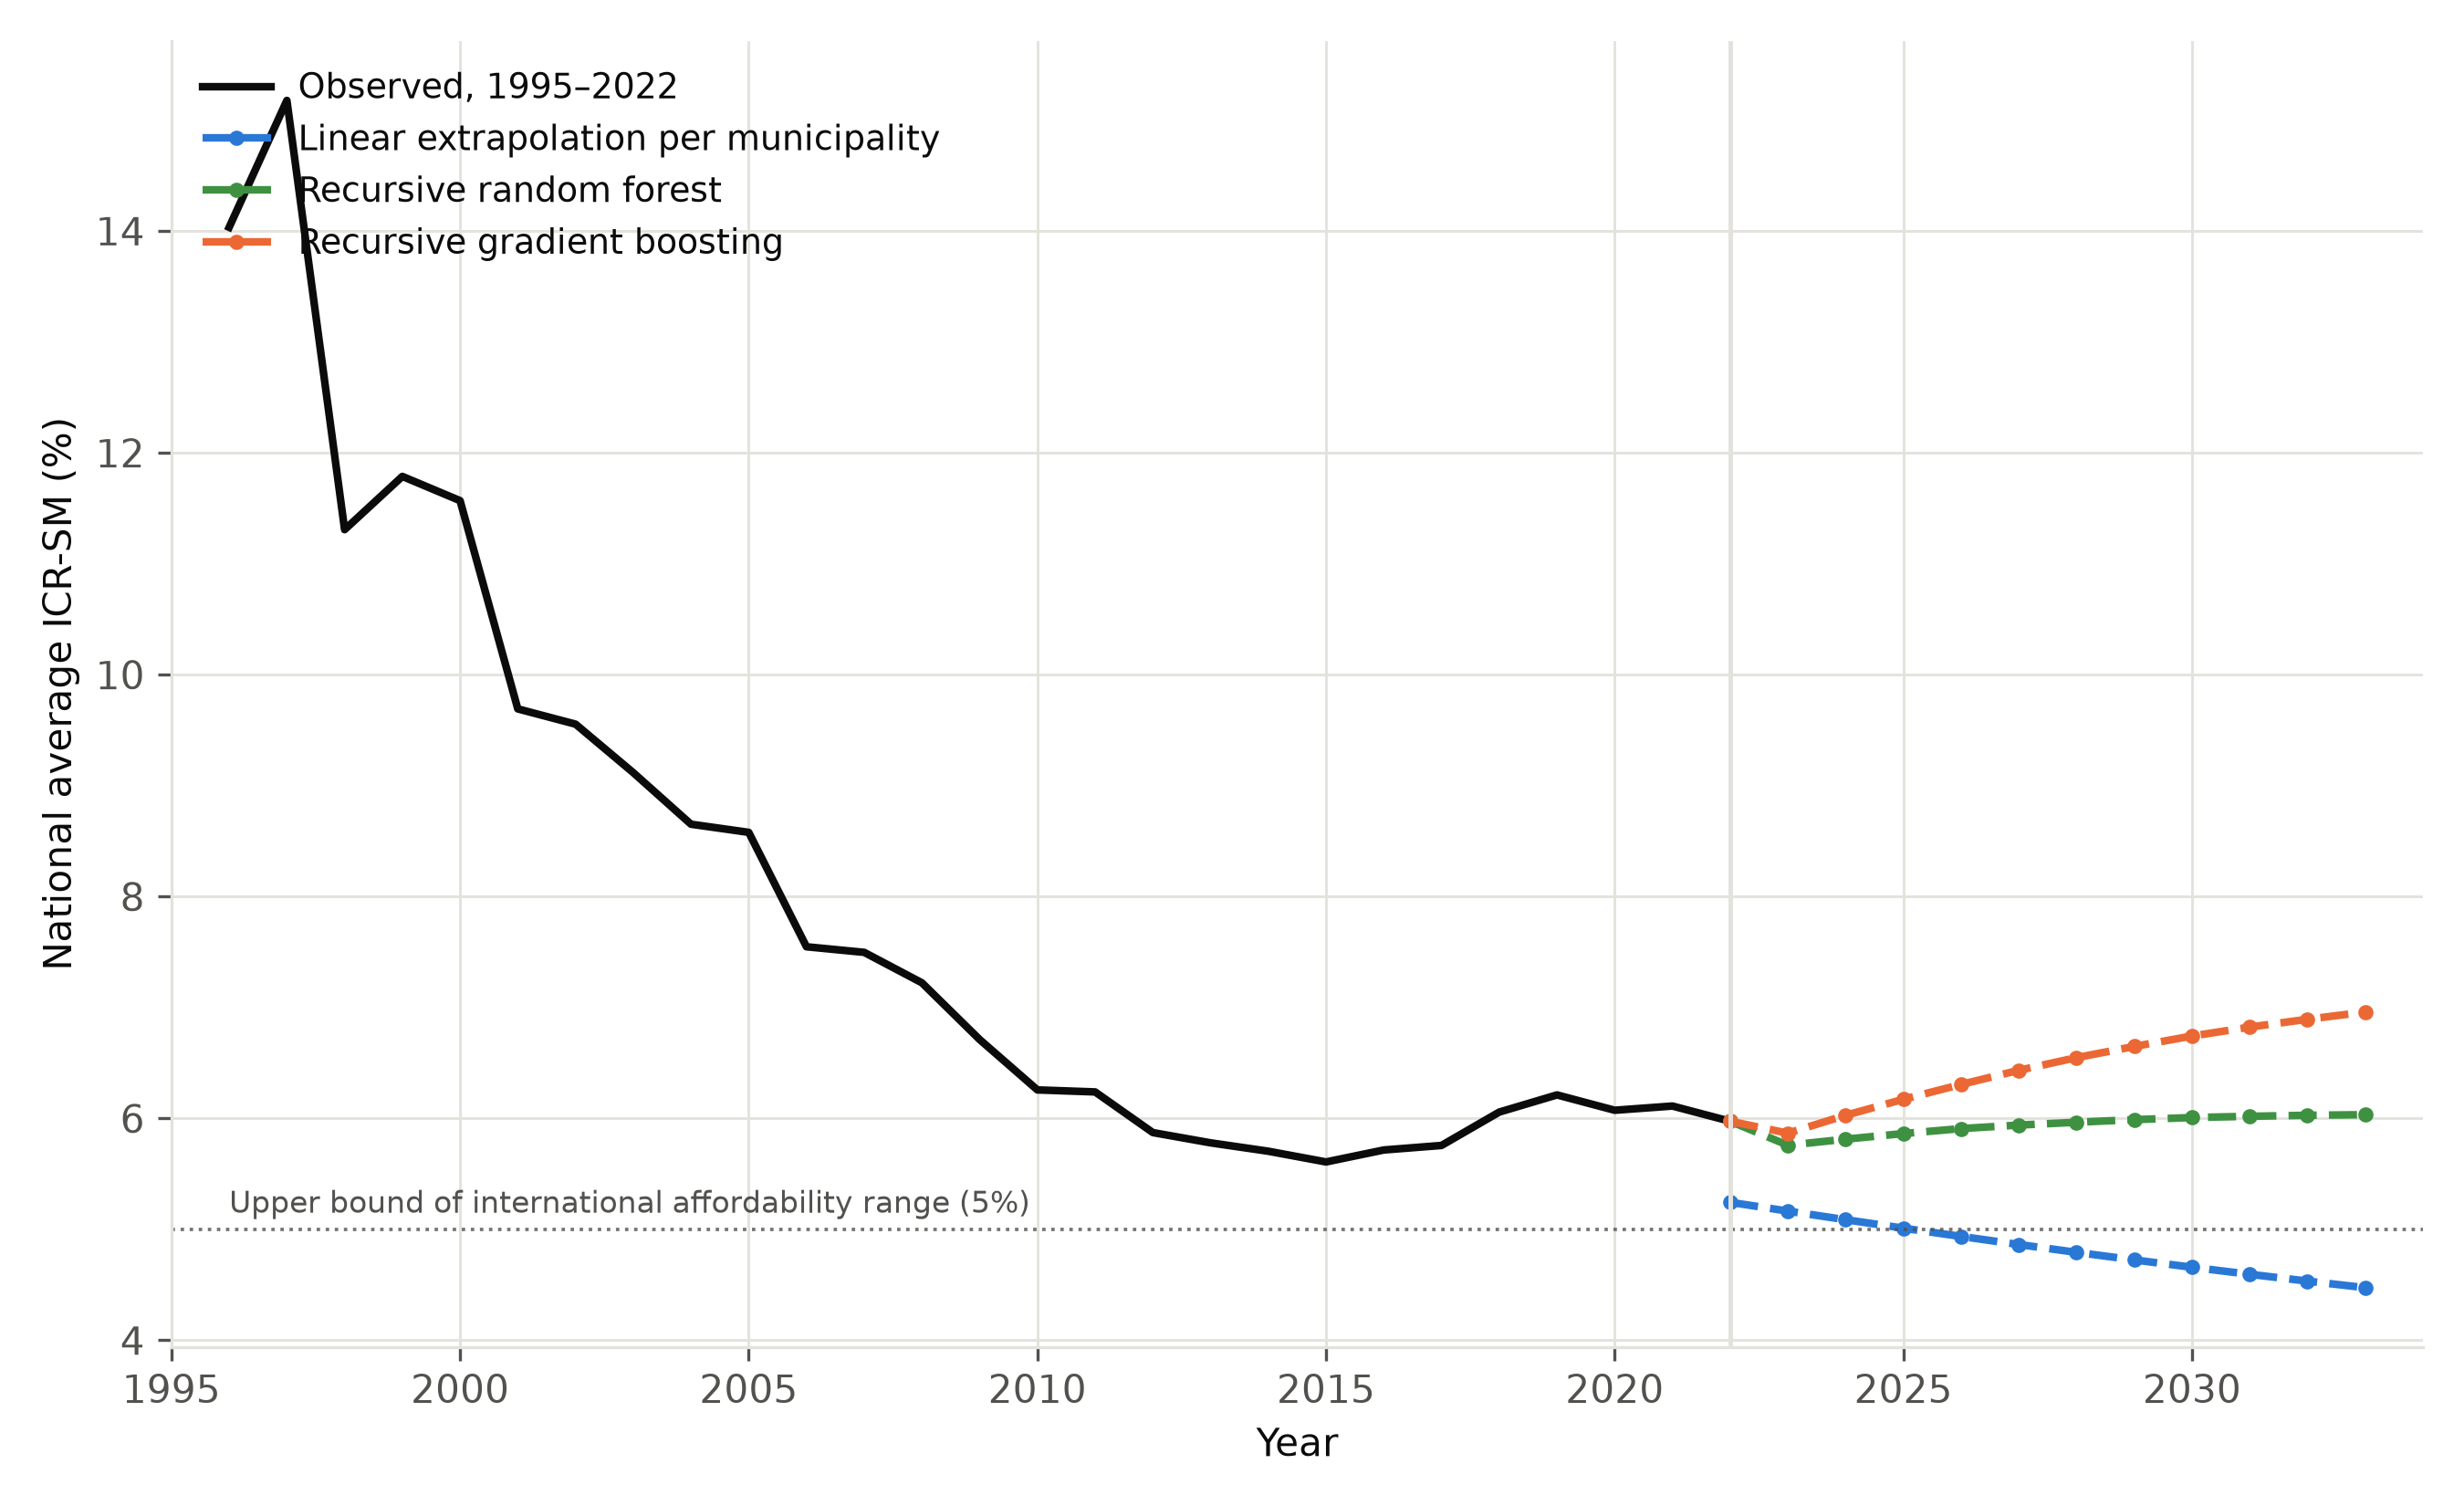
\includegraphics[width=0.85\textwidth]{../figuras/19_projecao_icr_2033.png}
\caption{National average ICR-SM, observed 1995 to 2022 and three conditional scenarios to 2033, a linear extrapolation of each municipality's own historical trend, a recursive random forest forecast and a recursive gradient boosting forecast. None of the three is validated as an eleven year forecast, they are sensitivity scenarios under different assumptions. The dotted horizontal line marks the 5 percent upper bound of the international affordability range used elsewhere in this paper.}\label{fig_icr_2033}
\end{figure}

None of the three scenarios should be read as the trajectory affordability will follow, and none is put forward as a central estimate or a likely range. They are conditional trajectories under different, explicit assumptions, offered to make the uncertainty in any 2033 statement about affordability explicit rather than to resolve it. Whether the tariff burden relative to the minimum wage improves or worsens by 2033 depends substantially on a policy variable, the future path of the minimum wage itself, that lies outside the four planning variables this paper tests and outside what any of these methods can resolve from the data alone.

Taken as a whole, this evidence is more consistent with affordability being shaped by conditions that are largely fixed within a municipality than with it being moved, year to year, by the specific planning choices captured in this panel, while coverage, and specifically the pace of coverage toward a legal deadline, appears more sensitive to demographic pressure and carries real forecasting uncertainty, uncertainty that is sharper still, and directional rather than merely a matter of degree, once the same exercise is applied to affordability itself. These are patterns observed in the data available for this study, not a closed account of what utility planning can or cannot achieve, and the next section discusses what they plausibly imply for how affordability planning should be understood and targeted.

\section{Discussion}\label{sec12}

The empirical picture assembled in the previous section speaks directly to the four questions that motivated it. Whether affordability responds, within the same municipality, to the level and stability of investment, the source of financing or the control of billing losses, the answer across every lagged specification tested on the full panel is that it does not in any way that current statistical power can detect, though Table~\ref{tab_periodo_2012_2022} shows this does not hold uniformly across the full period, and that qualification is carried forward rather than set aside. Heterogeneity across municipalities accounts for the overwhelming share of the variation in the income commitment ratio, while variation within a municipality over time, precisely the margin a manager or regulator can act on from one budget cycle to the next, accounts for almost none of it at an annual horizon. Read against the premise that opened this paper, that affordability is something utilities can be shown to produce through deliberate planning, the evidence available here does not support that premise, without establishing the stronger claim that affordability is causally fixed to place, a claim this panel, with its one year lag and its four reported planning variables, is not designed to test.

That reading also offers a plausible, though not directly tested, answer to why affordability planning is uncommon in practice, a puzzle noted at the outset. If the levers a utility can plausibly move in a given year in fact carry little weight against whatever is already fixed about a municipality, a possibility this panel is consistent with but cannot fully establish given its lag structure and variable set, then affordability planning would offer a comparatively poor return on managerial attention relative to measurement, which requires no behavioral change and produces a defensible number for a report. This is not an argument that planning is futile, only that the planning currently visible to the sector's own reporting system, and tested here on its own terms, does not show up as the lever. Where it might be, whether in provider governance, technical capacity, longer horizon investment effects, or forms of local political economy that the SNIS panel does not capture, remains open, and the large between municipality share of the variance is itself an invitation to look there next.

The regional and growth results answer the second and third questions and sharpen rather than soften that invitation. A trade off between expanding coverage and containing tariffs is real, but it is not a national phenomenon, it is concentrated in the North and the Central West, and notably absent where a simple story about catching up would predict it most, the Northeast. Growth pressure, in turn, divides cleanly along a line the introduction did not anticipate, it erodes coverage but leaves affordability untouched, and where it touches affordability at all, through faster growth in services, the association runs toward improvement rather than strain. Taken together, these two results imply that an equity agenda built around affordability cannot be a single national dial. It needs to be targeted at the specific regions where price and access genuinely compete, and at the specific pressure, demographic rather than financial, that coverage is actually exposed to.

The fourth question, whether water and sanitation share a trajectory toward the legal deadline, receives the least reassuring answer of the four. The two services are close to statistically independent in this sample, on track status in one carries little information about the other, and the regions that lead on water are not the regions that lead on sanitation. A regulatory framework that reports a single universalization date obscures that it is tracking two largely unrelated races, one of which, sanitation, is both further behind and measured on a substantially thinner reporting base. Any monitoring built on this legal target should report the two services separately rather than as a combined headline figure.

The forecasting exercise adds a dimension to this account that most of the affordability literature does not attempt, and it is worth dwelling on because the result is not simply that a more flexible model failed to help. Two forecasts were run with an identical architecture and holdout, one for water coverage and one for the affordability indicator itself, so the second speaks to the panel result directly rather than by analogy. Validated against a holdout period never seen during training, both gradient boosting models, trained on the full set of planning, economic and climate covariates, were outperformed by the simplest conceivable rule, repeating each municipality's last observed value. Permutation based ablation shows why in mechanical terms, the lagged outcome alone accounts for essentially all of each model's predictive accuracy, while most planning, economic and climate covariates contribute an amount indistinguishable from noise, with one partial exception, in the affordability model, log per capita GDP, lagged investment per capita, the lagged loss index and investment instability all show a small positive contribution that the coverage model does not show for any covariate. That contribution is far too small to overturn the panel finding that none of the four planning variables is individually significant, but it is a genuine, if modest, signal a purely linear fixed effects specification with a strict one year lag is not built to pick up, and it marks local economic conditions and investment level, rather than financing structure or billing losses, as the more promising place to look for a planning related channel at longer horizons. The predicted against observed comparison sharpens the main result further, in both models the fit is not merely no better than persistence, it is systematically worse at the extremes of the outcome distribution, pulling municipalities that are unusually far ahead or behind back toward the middle, the signature of a model with little genuine signal beyond the autocorrelation already present in the series. Read together, prediction rather than estimation, applied first to a different outcome and then to affordability directly, reaches the same substantive place as the panel regressions, the variables this sector reports about its own planning carry little detectable information, whether the question is asked by explaining past affordability or by forecasting future affordability or coverage. Reporting a projection to a legal deadline without first asking whether any model beats a naive benchmark, a step largely absent from prior work in this space, is offered here as a minimum bar for any future study that puts a date on universal access.

The question this special issue is ultimately organized around, what customer equity outcomes look like by the time universal access is due, cannot be answered with a single projected number for affordability, and that absence of a single answer is itself a substantive finding rather than a gap in the analysis. Extrapolating each municipality's own historical trend puts the national tariff burden back inside the international affordability range by 2033, consistent with two more decades of the real minimum wage appreciation documented earlier in this paper continuing on its historical path. Chaining either recursive machine learning model across the same horizon instead reverses the recent improvement, to 6.0 percent under random forest and 7.0 percent under gradient boosting, pushing the burden above that range for well over half of municipalities under either model. That the two machine learning models, sharing the same regressors and the same official demographic projection, still land almost a full percentage point apart is itself informative, it shows that part of the disagreement with the linear scenario reflects how a recursive forecast is built, boosting versus bagging, rather than only what it is built from. Because the panel evidence above shows the four planning variables tested here carry little detectable influence on affordability at a one year horizon, none of the three scenarios is itself a planning outcome in the sense this paper set out to test, all three are closer to different assumptions about how a variable this paper does not model, the future path of the minimum wage relative to tariffs, plays out over the next decade. The practical implication for monitoring this special issue's aim is that a 2033 affordability target, if one is adopted, should be tracked against several explicit, clearly labeled scenarios of this kind rather than against a single trend line or an implied central estimate, precisely because the drivers that would move the indicator lie mostly outside what utilities plan and report.

None of this is a claim that planning is beyond the reach of policy, only that the planning legible to this sector's information system does not, on the evidence gathered here, produce affordability outcomes on a yearly horizon. Two gaps in what that information system records remain open for future work. A national poverty registry, matched to this panel at the municipal level, could decompose part of the between municipality variance that this study leaves as an unexplained structural residual, testing directly whether local poverty rather than local planning is what the fixed effects are absorbing. The burden of initial connection costs, a dimension of access affordability distinct from the use affordability measured throughout this paper, also falls outside what the municipal SNIS panel records, and would extend the analysis from the price of an existing connection to the price of obtaining one in the first place.

Set against the aim of this special issue, the account that emerges is one in which the four planning instruments most readily reported by this sector show no robust association with the tariff burden in this panel, while a tariff burden gradient tied to municipal size and region, demographic pressure that falls on access rather than price, sector specific rather than joint targets, and forecasts honest about their own uncertainty, together point toward a different and more targeted equity agenda than the one the sector currently measures itself against.

\section{Conclusion}\label{sec13}

The objective of this study was to test whether the planning levers most often invoked in Brazilian water and sanitation policy, the level and stability of investment, the source of financing and the control of billing losses, explain variation in the tariff burden faced by connected customers across municipalities over time. This objective was pursued through a municipal panel spanning nearly three decades, estimated with municipality and year fixed effects so that the within municipality margin, the one a manager or regulator can actually act on from one budget cycle to the next, could be separated from the between municipality margin that reflects everything already fixed about a place. The objective was met in the narrow but load bearing sense that none of the four lagged planning variables shows a statistically robust within municipality association with the tariff burden, a result that recurs across four alternative specifications and an independent income denominator rather than depending on one particular choice, while heterogeneity across municipalities accounts for the large majority of the variation and the burden itself rises sharply with municipal size. Two forecasting exercises reinforce this reading with a different estimator and a different task, prediction rather than estimation. A gradient boosting model given the same planning, economic and climate covariates could not beat the naive rule of repeating each municipality's last observed value, whether the outcome forecast one year ahead was water coverage or the affordability indicator itself, and permutation importance shows the affordability forecast draws only a small, if genuine, signal from per capita GDP and investment level, not enough to alter the panel finding. Read together, these results are consistent with the four reported planning variables carrying limited information about either outcome at an annual horizon, though the panel cannot rule out that a longer lag, a different variable set, or provider level rather than municipal level detail would show more.

The remaining three research questions were answered along the way. The tariff burden rises close to monotonically with municipal population size, more than doubling between the smallest and the largest municipalities, a municipal-size tariff-burden gradient that none of the four planning variables tested here explains and that a future equity oriented monitoring framework should track directly rather than infer from national averages. A coverage affordability trade off exists but only in the North and the Central West, not as a national pattern. Population and economic growth pressure the access side of the system rather than the price side, eroding coverage while leaving affordability largely untouched. Water supply and sanitation follow largely independent trajectories toward the 2033 legal deadline, so that a municipality's standing on one service reveals little about the other, and any national monitoring framework built on a single combined target risks obscuring that divergence. Projecting the tariff burden itself to 2033 with a linear extrapolation and with two recursive machine learning models, gradient boosting and random forest, produces three conditional scenarios, not a validated forecast, that disagree in direction, not only in magnitude, the national average returns inside the international affordability range under the linear scenario and moves above it under both machine learning scenarios, by a smaller margin for random forest and a larger one for gradient boosting. None of the three is offered as a central estimate or a likely range, and given that the four planning variables tested here show little detectable influence on affordability at an annual horizon, this disagreement is best treated as an open question about 2033 rather than resolved in favor of any one method.

This account carries limitations that also set the agenda for future work. A one year lag rules out same year simultaneity but does not rule out reverse causality operating over a longer horizon, nor the possibility that municipalities anticipate future tariff or coverage pressure when they set investment, so the null result is best read as evidence against a fast, one year planning effect rather than against planning at every horizon. The four planning variables are also self reported administrative aggregates rather than direct measurements, so ordinary measurement error works against finding an association even where one exists, and the alternative income denominator check showed that the same variables do turn significant, with unexpected signs, when the sample is restricted to 2012 to 2022, an instability that is treated here as a genuine open question about the recent period rather than as fully resolved. The panel further captures only the planning variables that utilities report to the national information system, not every dimension of managerial or political practice that might influence the tariff burden, so the large between municipality variance documented throughout remains an unexplained structural residual rather than an identified cause, and a natural next step is to match this panel to a national poverty registry to test whether local income distribution rather than local planning is what the fixed effects absorb. The affordability measure used throughout also captures only the ongoing cost of an existing connection, saying nothing about the upfront cost of obtaining one, a distinct barrier that a future extension incorporating connection fees and informal settlement data could address. Finally, the forecast to 2033, like any extrapolation, assumes that the historical relationships estimated here continue to hold over a horizon more than twice as long as the holdout period used to validate it, a caveat that applies to every method compared in this paper and that argues for revisiting the projection as new years of data become available rather than treating it as a fixed answer.

\backmatter

\bmhead{Acknowledgements}

The authors thank the Coordenacao de Aperfeicoamento de Pessoal de Nivel Superior (CAPES) and the Universidade do Estado da Bahia (UNEB) for their support.

\section*{Declarations}

\begin{itemize}
\item \textbf{Funding.} This research received institutional support from CAPES and UNEB. No specific grant number applies.
\item \textbf{Conflict of interest/Competing interests.} The authors declare no competing interests.
\item \textbf{Ethics approval and consent to participate.} Not applicable. The study relies exclusively on publicly available, municipality and state level aggregated administrative and statistical records, with no human subjects, individual level data or personally identifiable information involved.
\item \textbf{Consent for publication.} Not applicable.
\item \textbf{Data availability.} All source data are publicly available. The utility panel comes from the National Sanitation Information System (SNIS), Brazil's Ministry of Cities. The minimum wage series combines the IBGE historical record and an independent cross check at Contabeis.com.br. Municipal GDP and population come from IBGE SIDRA tables 5938 and 6579. The precipitation series is built from the Open-Meteo historical weather archive. State level average wages for the robustness check come from the PNADC household survey. The official 2022 to 2033 population growth projection used in the recursive affordability forecast comes from IBGE SIDRA table 7358. Exact access points are given as footnotes in Section~\ref{subsec_data}, Section~\ref{subsec_resultados5} and in Table~\ref{tab_sources}. Smaller intermediate results, including all model output files, coefficient tables and 2033 projection files, are archived together with the code at \url{https://doi.org/10.5281/zenodo.21968533}. The constructed municipal panel and other raw or intermediate files too large for a code repository are available from the corresponding author upon reasonable request.
\item \textbf{Materials availability.} Not applicable.
\item \textbf{Code availability.} The full analysis pipeline is implemented as a sequence of independent, numbered scripts covering panel construction, the panel regression models, the robustness checks, the machine learning forecast and validation, and all figures, as described in Section~\ref{subsec_panel_spec}. The scripts, a README describing the execution order and package versions, and the recorded random seeds are archived on GitHub and Zenodo, \url{https://doi.org/10.5281/zenodo.21968533}.
\item \textbf{Author contribution.} All authors contributed to the study conception, design, analysis and writing, and approved the final manuscript.
\end{itemize}

%%===================================================%%
%% For presentation purpose, we have included        %%
%% \bigskip command. Please ignore this.             %%
%%===================================================%%
\bigskip
\begin{flushleft}%
Editorial Policies for:

\bigskip\noindent
Springer journals and proceedings: \url{https://www.springer.com/gp/editorial-policies}

\bigskip\noindent
Nature Portfolio journals: \url{https://www.nature.com/nature-research/editorial-policies}

\bigskip\noindent
\textit{Scientific Reports}: \url{https://www.nature.com/srep/journal-policies/editorial-policies}

\bigskip\noindent
BMC journals: \url{https://www.biomedcentral.com/getpublished/editorial-policies}
\end{flushleft}

% \begin{appendices}

% \section{Section title of first appendix}\label{secA1}

% An appendix contains supplementary information that is not an essential part of the text itself but which may be helpful in providing a more comprehensive understanding of the research problem or it is information that is too cumbersome to be included in the body of the paper.

% %%=============================================%%
% %% For submissions to Nature Portfolio Journals %%
% %% please use the heading ``Extended Data''.   %%
% %%=============================================%%

% %%=============================================================%%
% %% Sample for another appendix section			       %%
% %%=============================================================%%

% %% \section{Example of another appendix section}\label{secA2}%
% %% Appendices may be used for helpful, supporting or essential material that would otherwise 
% %% clutter, break up or be distracting to the text. Appendices can consist of sections, figures, 
% %% tables and equations etc.

% \end{appendices}

%%===========================================================================================%%
%% If you are submitting to one of the Nature Portfolio journals, using the eJP submission   %%
%% system, please include the references within the manuscript file itself. You may do this  %%
%% by copying the reference list from your .bbl file, paste it into the main manuscript .tex %%
%% file, and delete the associated \verb+\bibliography+ commands.                            %%
%%===========================================================================================%%

\bibliography{sn-bibliography}% common bib file
%% if required, the content of .bbl file can be included here once bbl is generated
%%\input sn-article.bbl

\end{document}
